\documentclass{nst}

\usepackage{dcolumn}
\usepackage[T2A,T1]{fontenc}
\usepackage[russian,english]{babel}
\usepackage{comment}
\usepackage{subcaption}
\usepackage{caption}

% The following package will be used to typeset the LaTeX codes and is not a necessity to this template
\usepackage{listings}
\lstloadlanguages{[LaTeX]TeX}
\lstset{language=[LaTeX]TeX,keywordstyle=\color{red},showspaces=true,breaklines=true,breakatwhitespace=true,basicstyle=\small\tt,commentstyle=\color{white},frame=single,framerule=0pt,backgroundcolor=\color{yellow}}


\begin{document}


\title{A versatile test bench for photomultiplier tube characterization and its application in the DAMPE-PSD}\thanks{Supported by the Strategic Priority Research Program of the Chinese Academy of Science~(No. XDA04040202-3)}

\author[周勇]{ZHOU Yong}
\affiliation{Institute of Modern Physics, Chinese Academy of Sciences, 509 Nanchang Road, Lanzhou, 730000, P.R.China}
\affiliation{School of Nuclear Science and Technology, Lanzhou University, 222 South Tianshui Road, Lanzhou, 730000, P.R.China}
\affiliation{Graduate University of the Chinese Academy of Sciences, 19A Yuquan Road, Beijing, 100049, P.R.China}
\author[孙志宇]{SUN Zhi-Yu}
\affiliation{Institute of Modern Physics, Chinese Academy of Sciences, 509 Nanchang Road, Lanzhou, 730000, P.R.China}
\author[余玉洪]{YU Yu-Hong}
\email[Corresponding author, ]{yuyuhong@impcas.ac.cn}
\affiliation{Institute of Modern Physics, Chinese Academy of Sciences, 509 Nanchang Road, Lanzhou, 730000, P.R.China}
\author[张永杰]{ZHANG Yong-Jie}
\affiliation{Institute of Modern Physics, Chinese Academy of Sciences, 509 Nanchang Road, Lanzhou, 730000, P.R.China}
\author[方芳]{FANG Fang}
\affiliation{Institute of Modern Physics, Chinese Academy of Sciences, 509 Nanchang Road, Lanzhou, 730000, P.R.China}
\author[陈俊岭]{CHEN Jun-Ling}
\affiliation{Institute of Modern Physics, Chinese Academy of Sciences, 509 Nanchang Road, Lanzhou, 730000, P.R.China}
\author[胡碧涛]{HU Bi-Tao}
\affiliation{School of Nuclear Science and Technology, Lanzhou University, 222 South Tianshui Road, Lanzhou, 730000, P.R.China}


\begin{abstract}
 Performance characterization for massive photomultiplier tubes (PMT) is a frequently encountered procedure in large nuclear and particle experiments. To facilitate this work, a dedicated test bench system has been developed at the Institute of Modern Physics, Chinese Academy of Sciences.
 The two-dimensional photocathode position scanning capability is an intrinsic function of the test bench and up to 25 PMTs, with the diameter smaller than 2", can be tested simultaneously.
 The parameters of the light source pulses can be adjusted in a wide range, thus making it suitable for various characteristics measurements.
 The test bench system is highly automated with all the controlling operations integrated into a single software. 
 Additionally, the hardware platform is extensible which allows complex testing schemes, and the modularity in the software design make the migration from one testing configuration to another light-weight and efficient.
 All these features make the test bench versatile and reusable in different experiments.
 It has been first used in the construction of the Plastic Scintillator Detector (PSD) of DArk Matter Particle Explorer (DAMPE), and a total of 570 Hamamatsu R4443 tubes were tested successfully. The performance was verified and the testing results are also reported in this aritcle.
\end{abstract}


\keywords{Photomultiplier tube, Large detector systems for particle and astroparticle physics, Test bench system, DAMPE-PSD}

\maketitle


\section{Introduction}
\label{sec:introduction}

Since their invention about 80 years ago, photomultiplier tubes (PMTs) have been widely used as photosensors in nuclear and particle physics experiments due to the high sensitivity, fast time response and other inherent benefits. 
Today, large-scale experiments may contain thousands of PMTs or more. To achieve optimal detector performance, it's important to characterize each PMT before they are put into usage. 
%Manufacturers provide datasheets with parameters that are normally used in the industry, but may not be useful or applicable for physics experiments.
Sometimes, general information provided by manufacturers is not particularly useful for a specific experiment.
On the other hand, some experiments may have special requirements on certain characteristics of the PMTs that are absent from the datasheets. 
Therefore, characterization of PMTs is a mandatory step in setting up large-scale experiments.

Characterizing a large number of PMTs in limited time is a challenging job. Usually a dedicated test bench is constructed to facilitate this work~\cite{barnhill_testing_2008,akgun_complete_2005,adragna_pmt-block_2006}.
Setting up a system like this is not trivial work. It requires investment of considerable amount of time and effort.
On the other hand, testing of PMTs is a common task and many components of the testing configuration can be shared among different applications.
Thus, it is beneficial to build a single modular PMT test system that could be easily reconfigured for various experiments.

In this paper, a versatile test bench dedicated for characterization of large amount of PMTs is described.
The test bench is designed to be a standard laboratory equipment for the PMT characterization tasks of several experiments prepared and planned at the Institute of Modern Physics (IMP), Chinese Academy of Sciences (CAS).
To accommodate various requirements of different experiments and make the test bench reusable in different applications, great attention has been paid to the selection of  hardware components and the design of the software framework (see Section~\ref{sec:description}).
The first user of this test bench is the Plastic Scintillator Detector (PSD), a sub-detector of the DArk Matter Particle Explorer (DAMPE)~\cite{Chang_Jin_dampe} which is a satellite-borne experiment. 
Characterization of PMTs for PSD using this test bench was very successful. The performance of the test bench has been demonstrated.
Summary of the test results are presented in Section~\ref{sec:application}.

\section{Description of the test bench}
\label{sec:description}

\begin{figure*}[!htb]
	\centering
	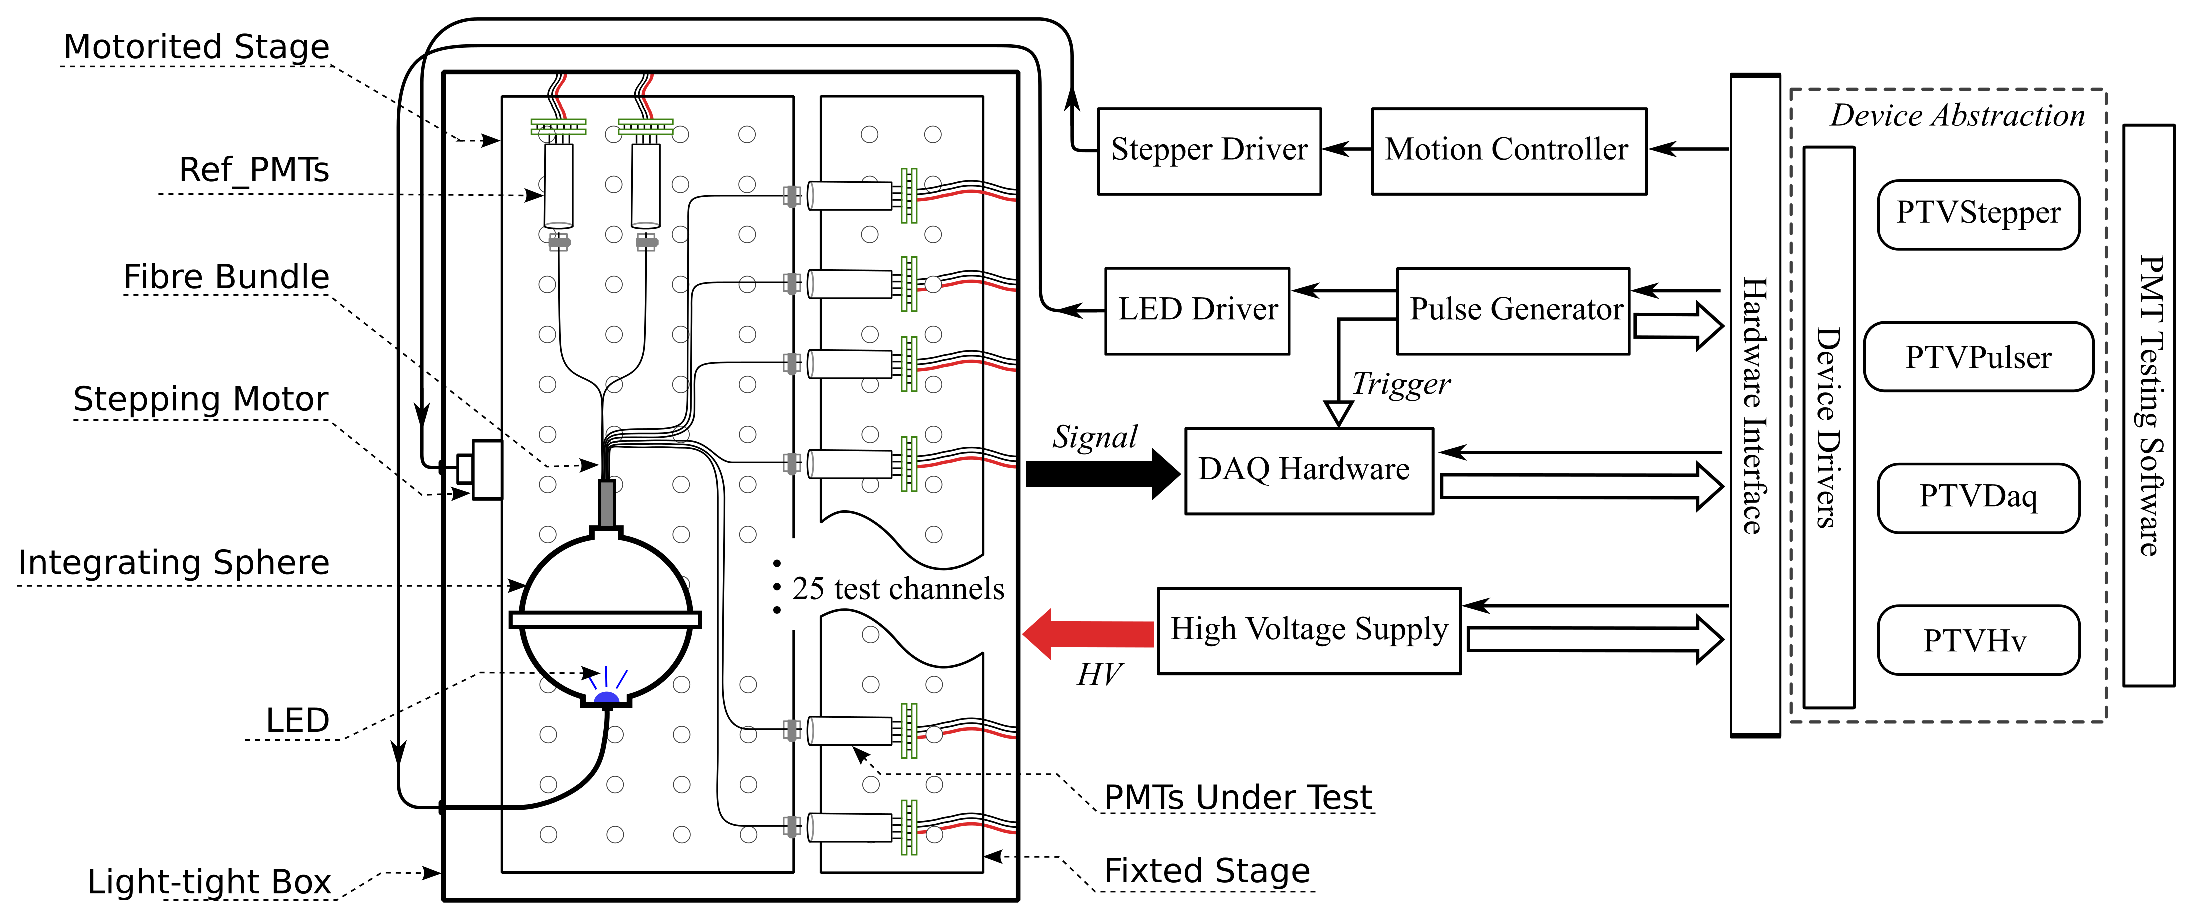
\includegraphics[width=150mm]{FIG1}
	\caption{Schematic diagram of the PMT test bench system.}
	\label{fig:FIG1}
\end{figure*}

The characteristics of the test bench can be summarized as follows:
\begin{itemize}
	\item \textit{Large capacity}: This is the primary driving force for developing a test bench dedicated for PMT characterization.
	Testing multiple tubes simultaneously can increase the efficiency tremendously, and this is a critical factor in projects involving a large number of PMTs. 
	\item \textit{Automation}: A single test run for PMT characterization usually takes several hours. Most steps of this process are routine operations such as changing voltage, sweeping light intensity and so on.
	Manual operations are inefficient and unreliable in such a long period.
	Computer controllable hardware is preferred in building the test bench, and corresponding software has been developed to automate common routine operations.
	Human intervention is only expected at the beginning of the test run when mounting the PMTs and configuring the software, and at the end of the run when unmounting the PMTs and assessing the test results.
	\item \textit{Versatility}: Various potential use cases have been considered in the design of the test bench, specifically the cathode scanning capability was incorporated as an intrinsic function of the test bench.
	Appropriate hardware has been set up in the first place, and general-purpose devices were adopted whenever possible.
	\item \textit{Flexibility}: %Flexibility is realized both in terms of hardware and software based on the modularity principle.
	The hardware platform is expandable and the components are loosely coupled, thus allowing complex testing configurations and convenient replacement or upgrade of the hardware.
	The software was carefully designed to provide abstract interfaces for device control. Thus, swapping hardware components has little impact on the high level functionality. This makes the software compatible across platforms.
	%The software abstracts the device control operations and the changing of hardware is handled smoothly in the software design, keeping the high level functionality unchanged and portable. 
\end{itemize}

A schematic diagram of the PMT test bench is shown in Fig.~\ref{fig:FIG1}.
Up to 25 PMTs can be characterized at the same time.
Light pulses from a blue light emitting diode (LED) are distributed to the PMTs through an integrating sphere and a transparent fiber bundle, which are mounted on a three-axes motorized stage.
PMTs under test are mounted on a separate fixed stage. This allows one to scan the photocathodes of all PMTs simultaneously.
There are also two monitoring PMTs fixed on the motorized stage.
Their positions remained unchanged relative to the input fiber in all operations and they were used to monitor the stability of the LED as well as the performance of the test bench system.
Both stages are housed in a black light-tight container made of aluminum alloy (see Fig.~\ref{fig:FIG2_a}), with a dimension of $176cm\times100cm\times78cm$.
%The container is painted black inside and the lid can be removed for operations such as tube mounting.

For the proper operation of the test bench, a variety of auxiliary devices are needed. 
They are divided into four functional groups according to the functions they provide: motion control (including the stepper driver), pulse generation (including the LED driver), high voltage supply and data acquisition (DAQ).
The devices for motion control and pulse generation are tightly coupled to the test bench itself, thus the same hardware can be reused for nearly all the use cases.
On the other hand, the devices for DAQ and high voltage supply are closely related to the intended large-scale experiment which needs PMT characterization, and project-specific hardware is often chosen in different experiments.
%The changing of hardware is handled smoothly in the software design, which will be discussed in more detail in Section~\ref{sec:software}.
Originally, a universal CAEN SY1527LC~\cite{sy1527lc} power crate was adopted as the high voltage supply system and a CAMAC crate with the CC-USB crate controller~\cite{cc_usb} was used for the DAQ.
All the auxiliary devices were placed outside the light-tight container, and the cables were led out through light-tight feedthroughs.
%The control of all these equipments are integrated into a single software. The changing of hardware is handled smoothly in the software design and automation is realized in every aspect of the test bench.

The whole test bench sits in an ISO class 8 cleanroom at IMP, and the room temperature is kept to be $22\pm2$\si{\celsius}~all the time. 
In the following sections, the key components of the test bench are described in detail.

\subsection{Motorized and fixed stages}
\label{sec:stages}

\begin{figure}[!htb]
	\begin{subfigure}[t]{80mm}
		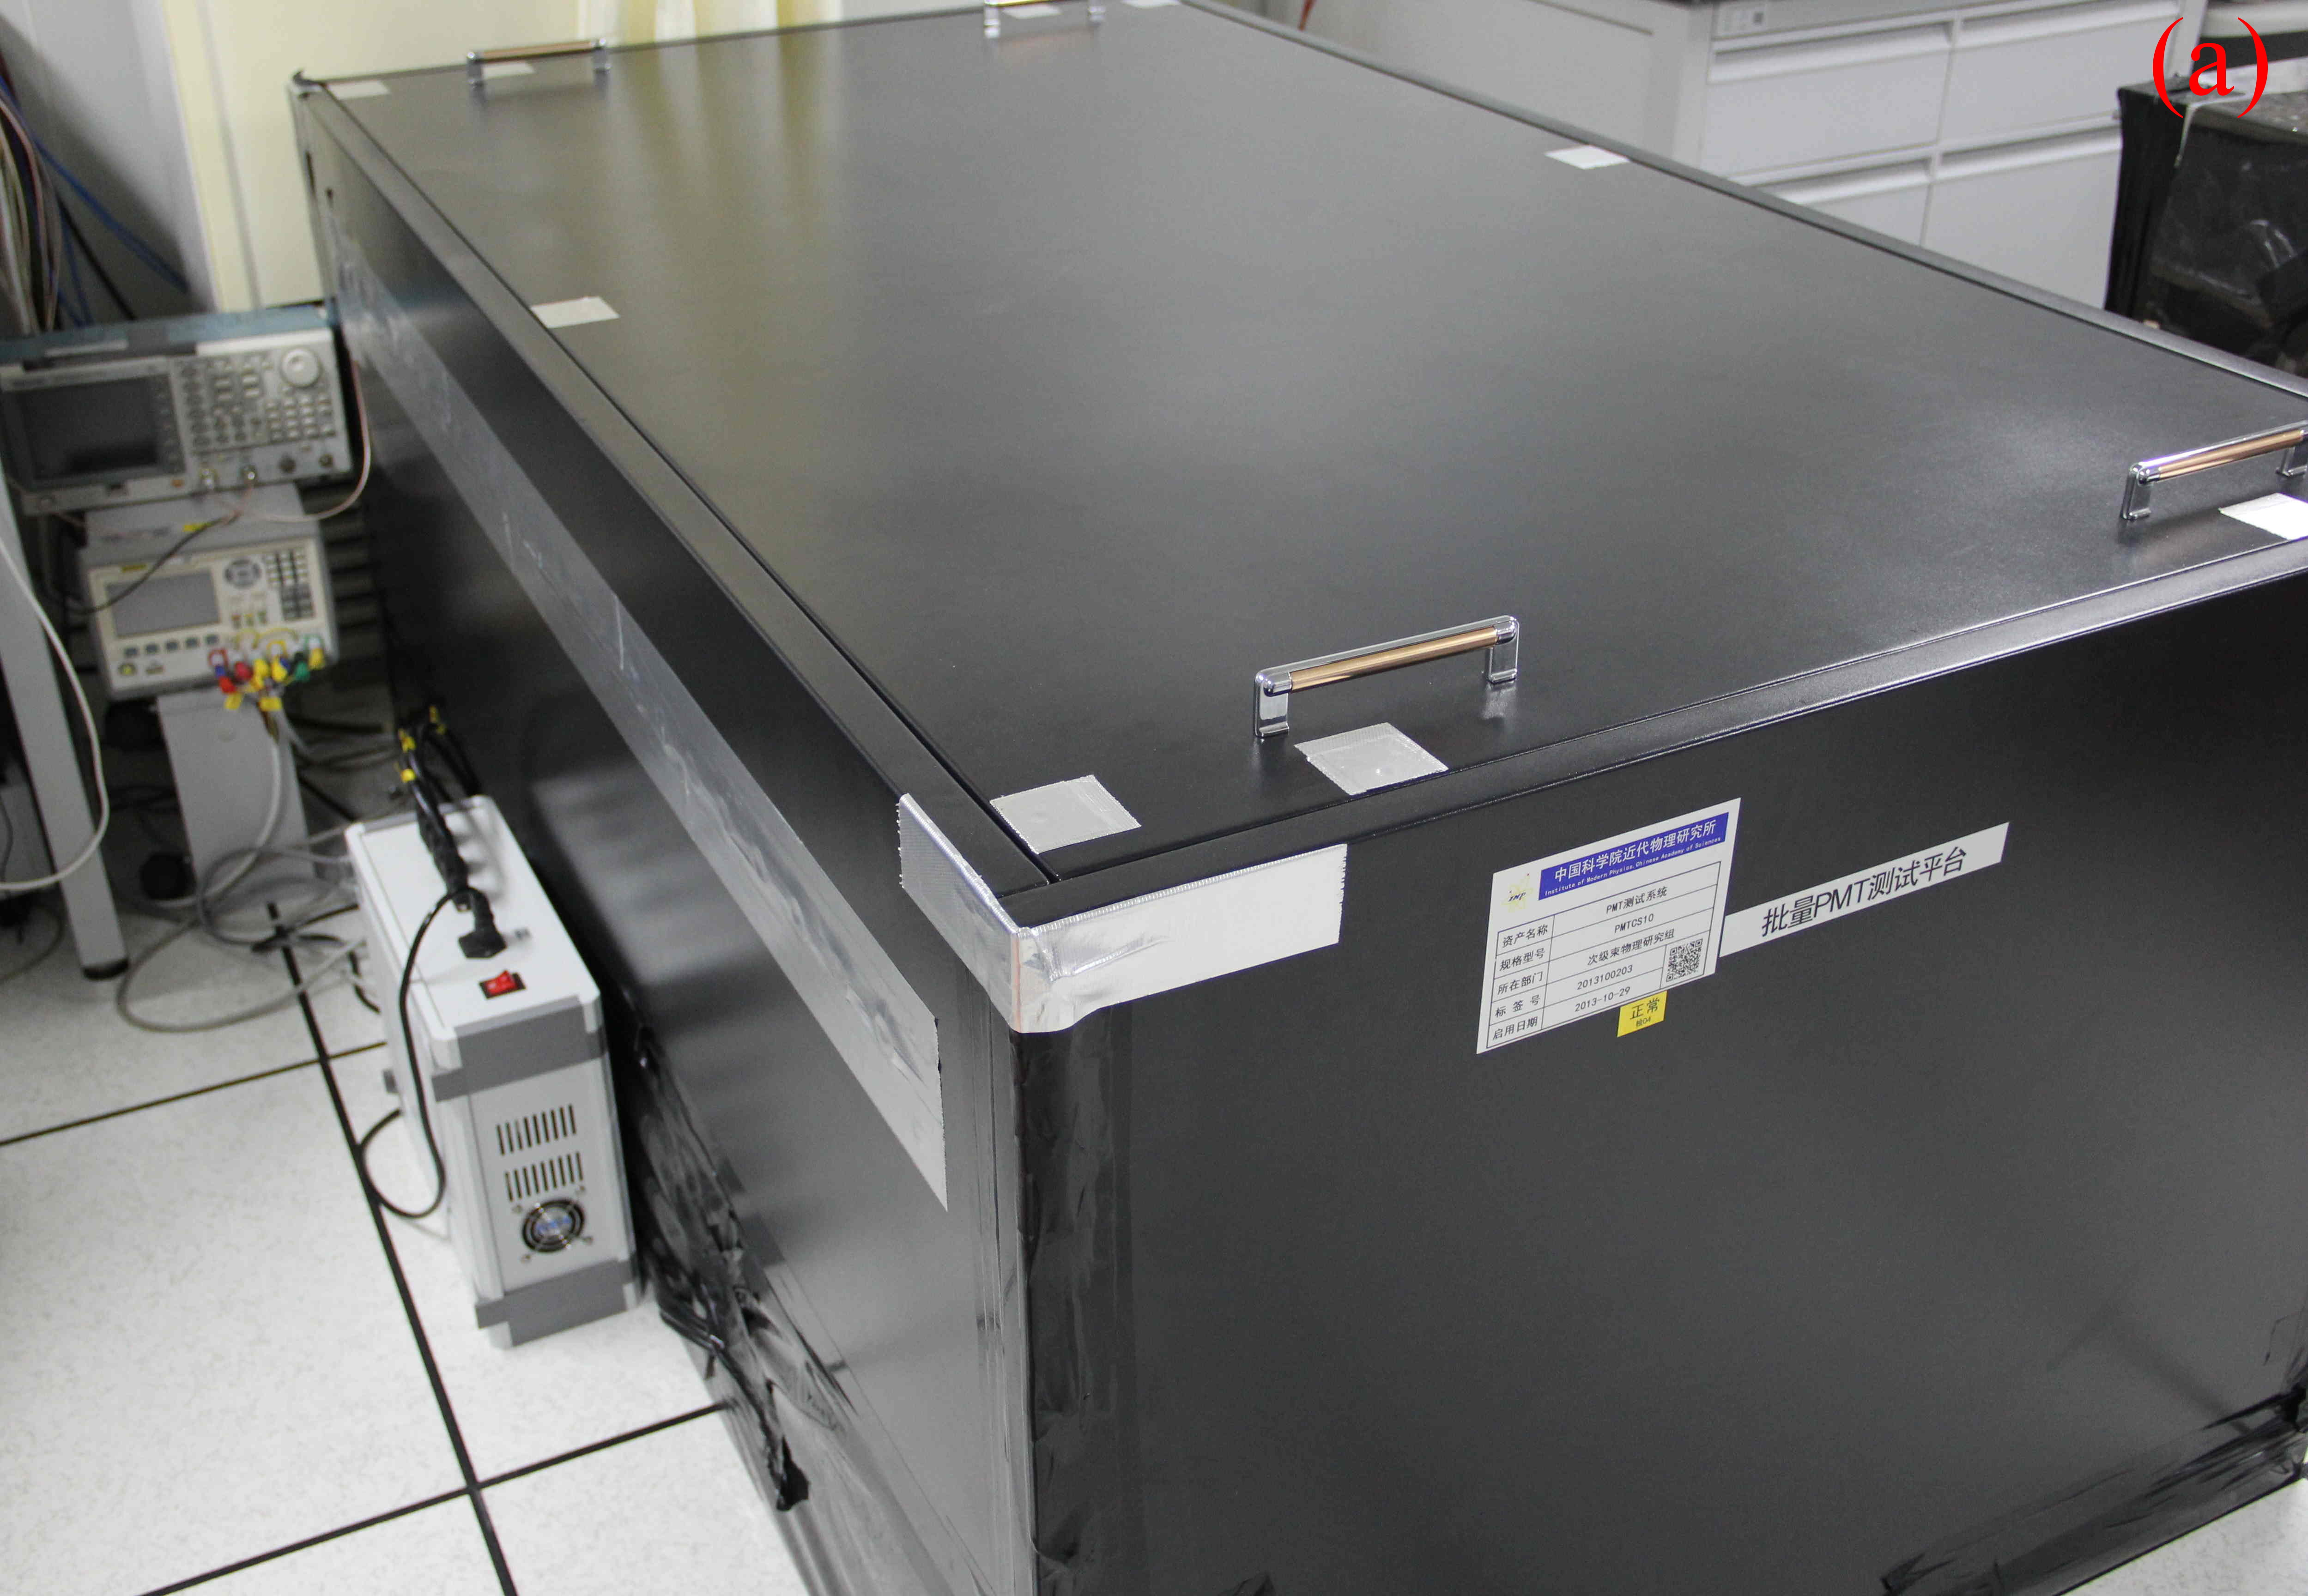
\includegraphics[width=80mm]{FIG2_a}
		\caption{Light-tight container.}
		\label{fig:FIG2_a}
	\end{subfigure}
	\begin{subfigure}[t]{80mm}
		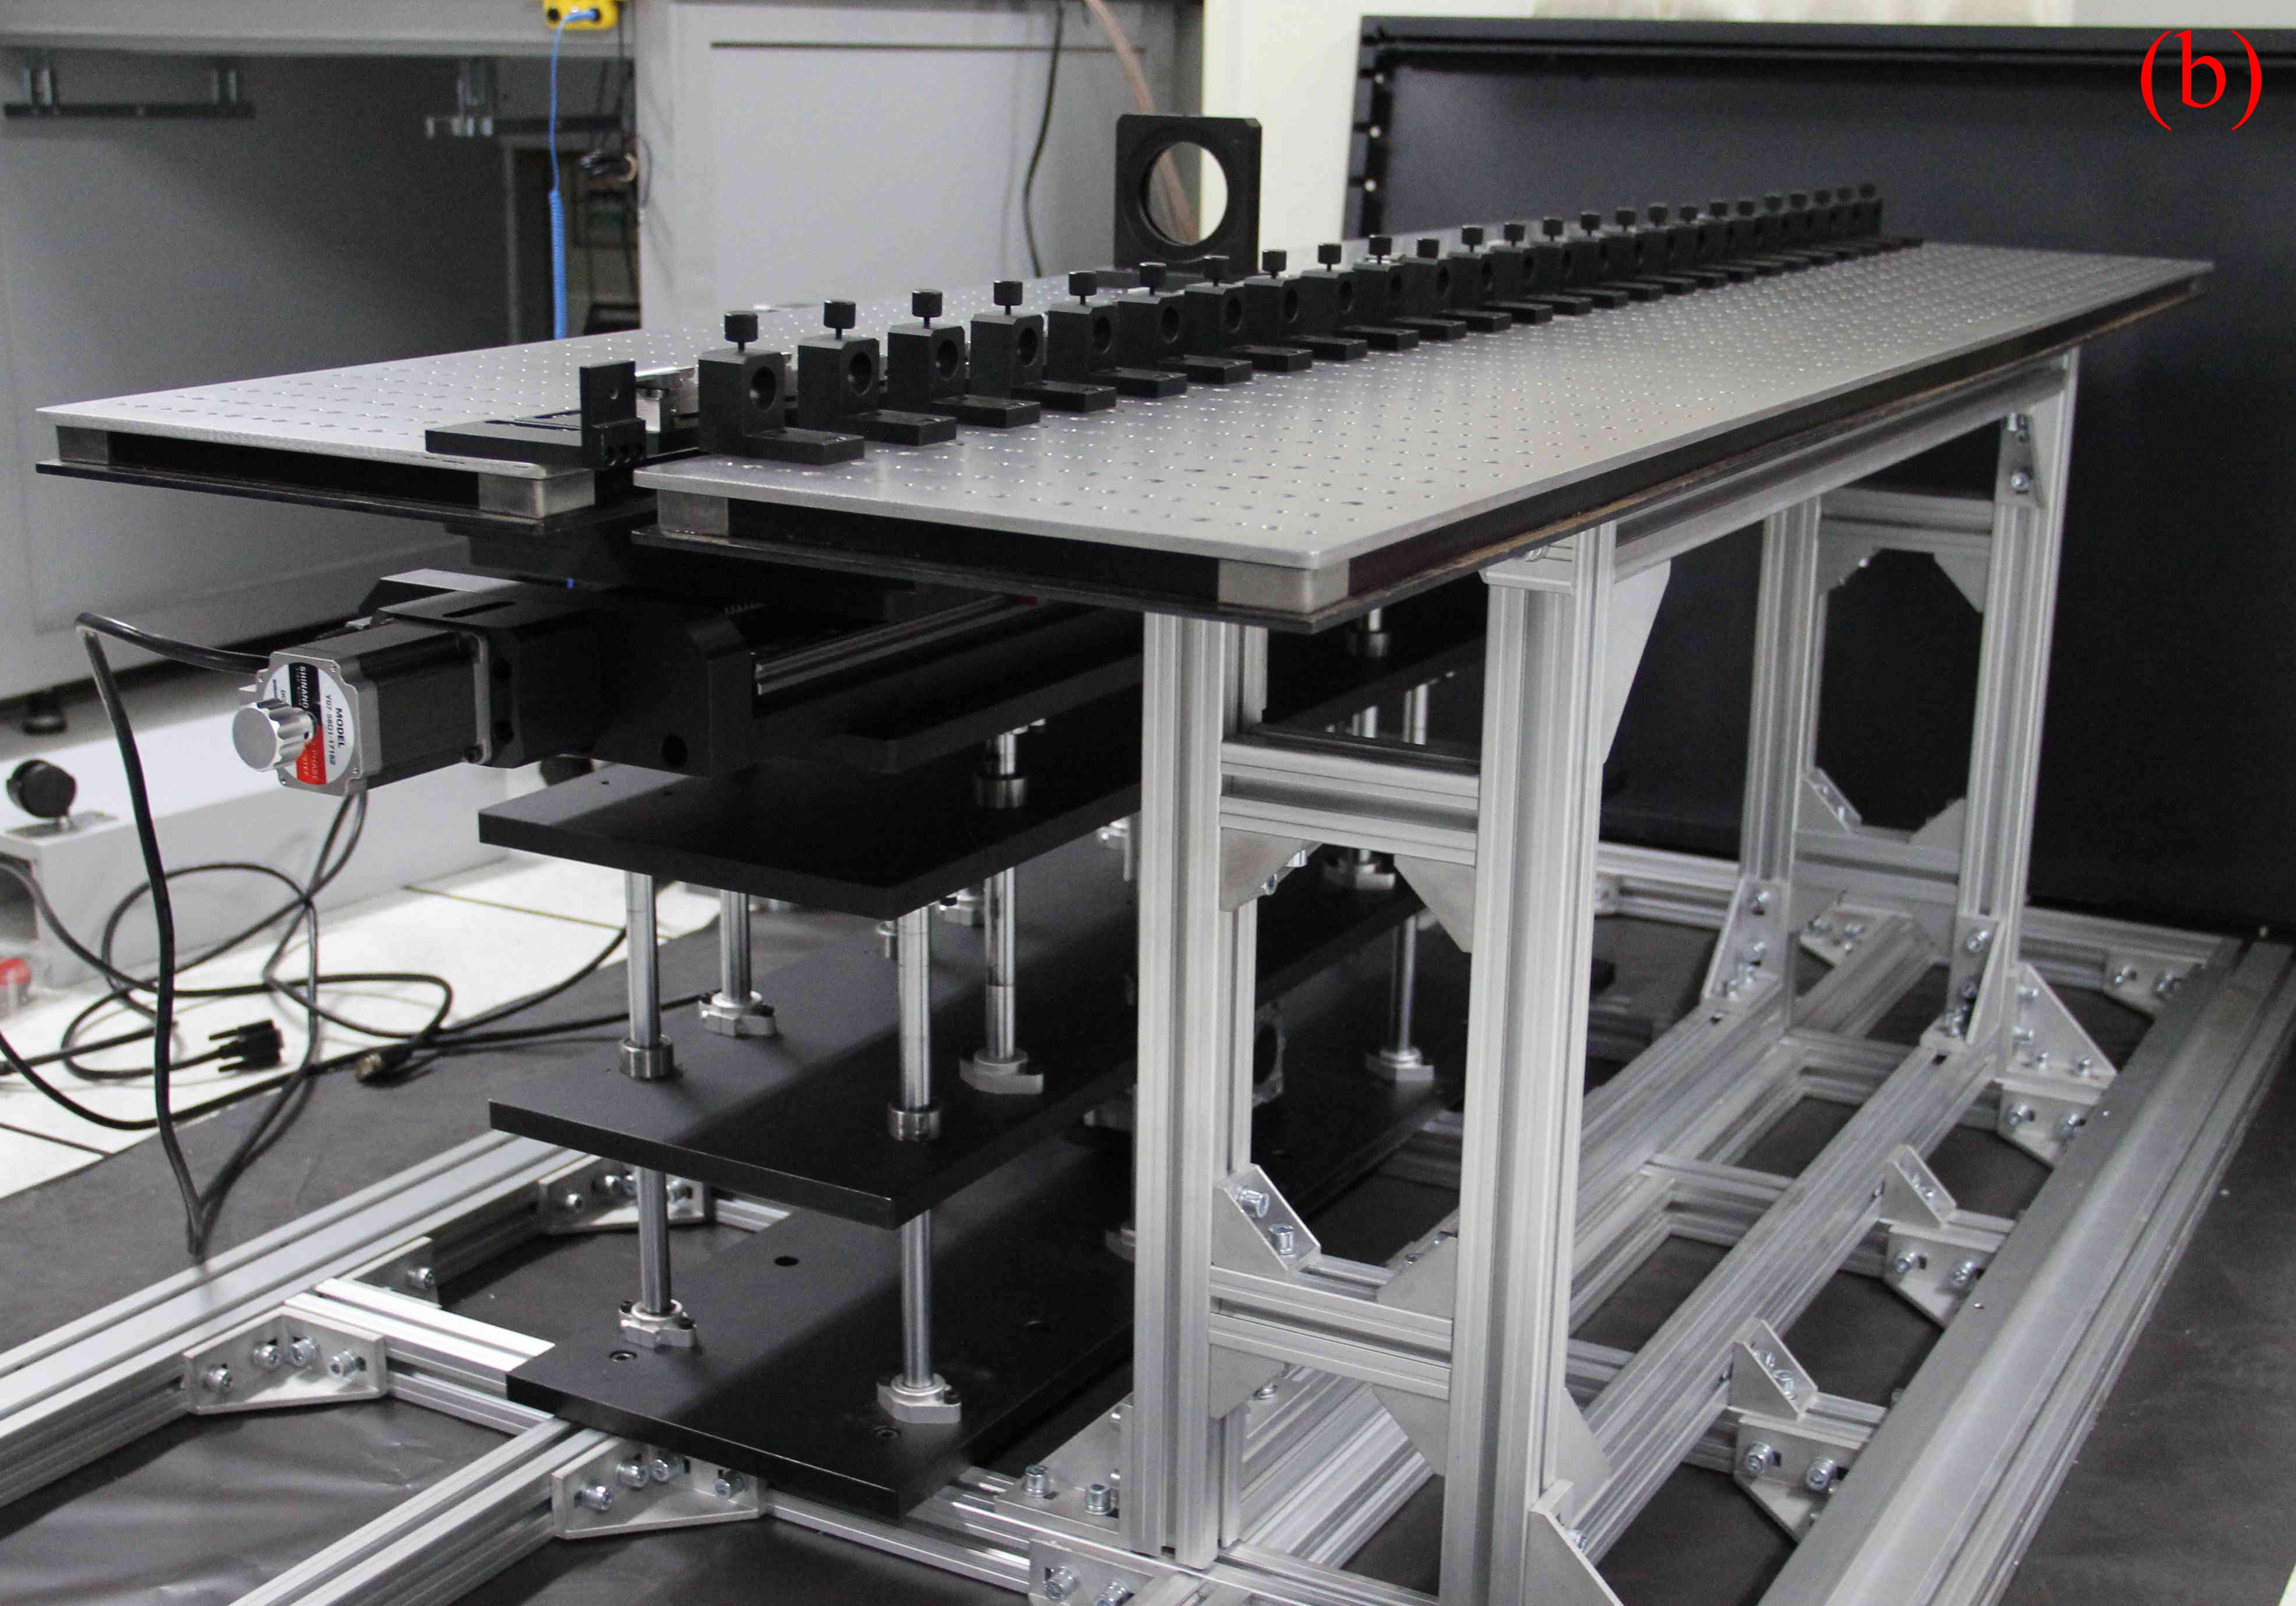
\includegraphics[width=80mm]{FIG2_b}
		\caption{Motorized and fixed stages before assembly.}
		\label{fig:FIG2_b}
	\end{subfigure}
	\caption{Main body of the PMT test bench.}
	\label{fig:FIG2}
\end{figure}

\begin{figure}[!htb]
	
	\begin{subfigure}[t]{80mm}
		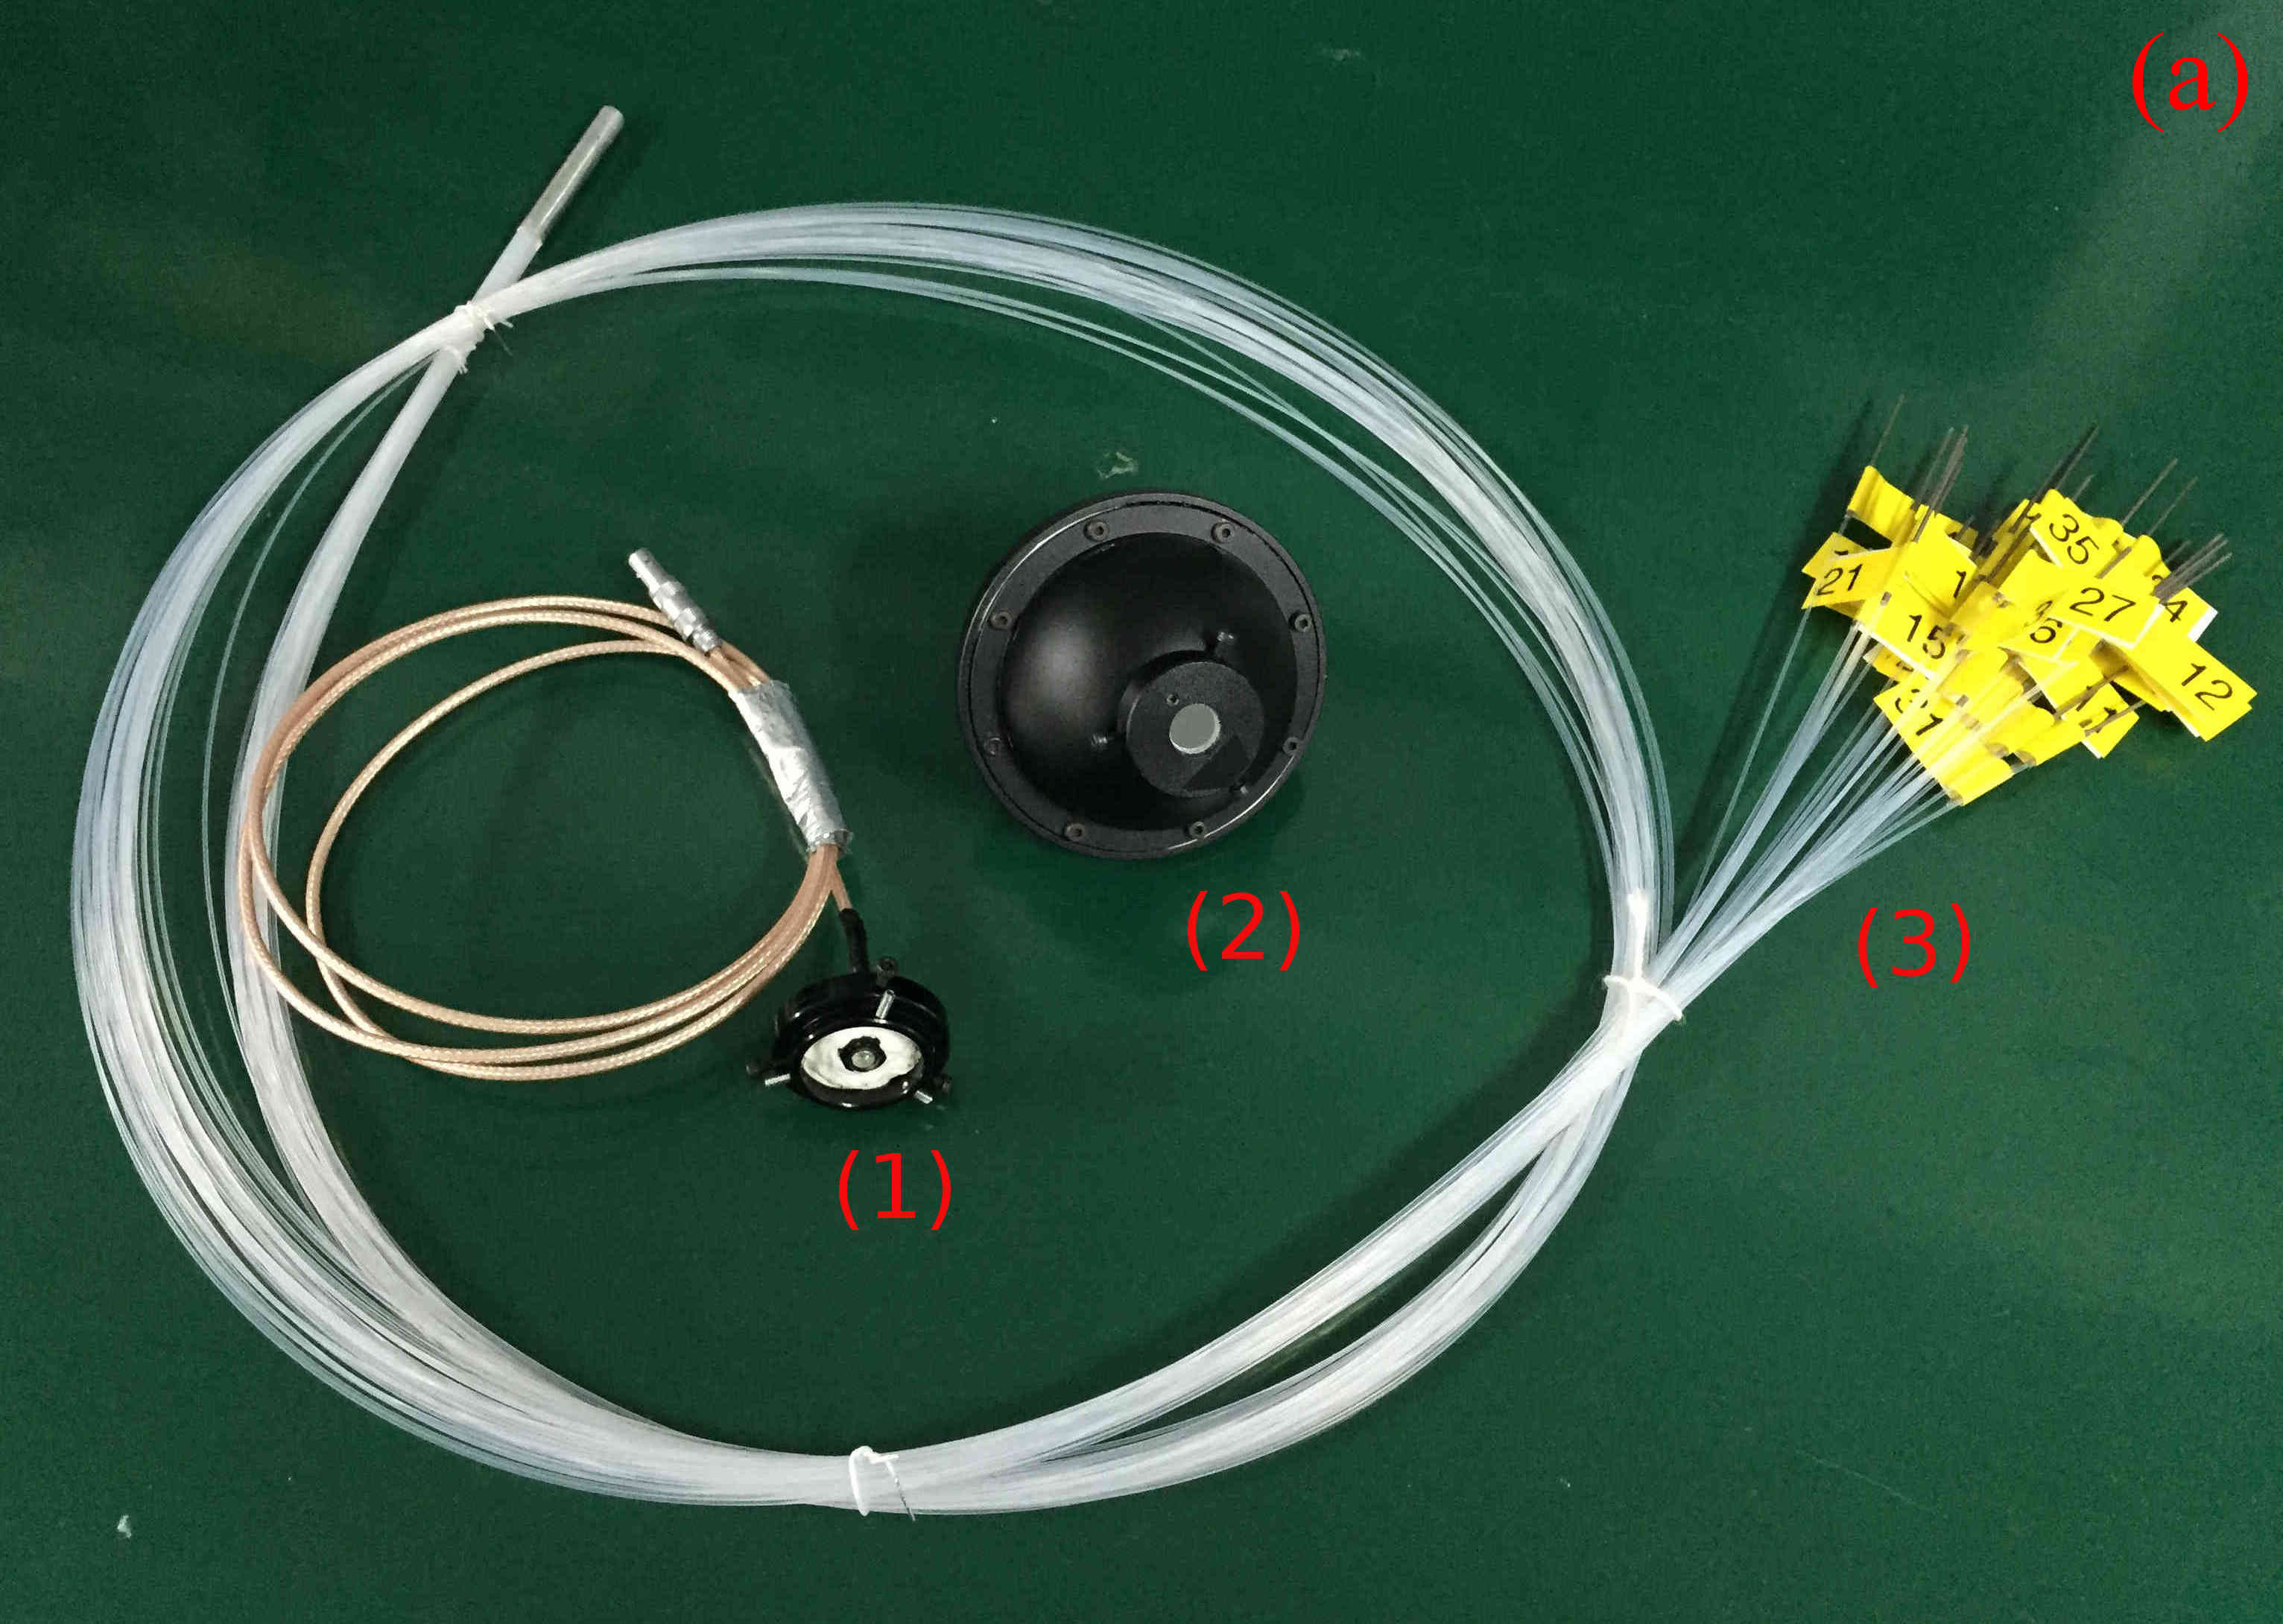
\includegraphics[width=80mm]{FIG3_a.jpg}
		\caption{1) LED; 2) Integrating sphere; 3) Fiber bundle}
		\label{fig:FIG3_a}
	\end{subfigure}
	\begin{subfigure}[t]{80mm}
		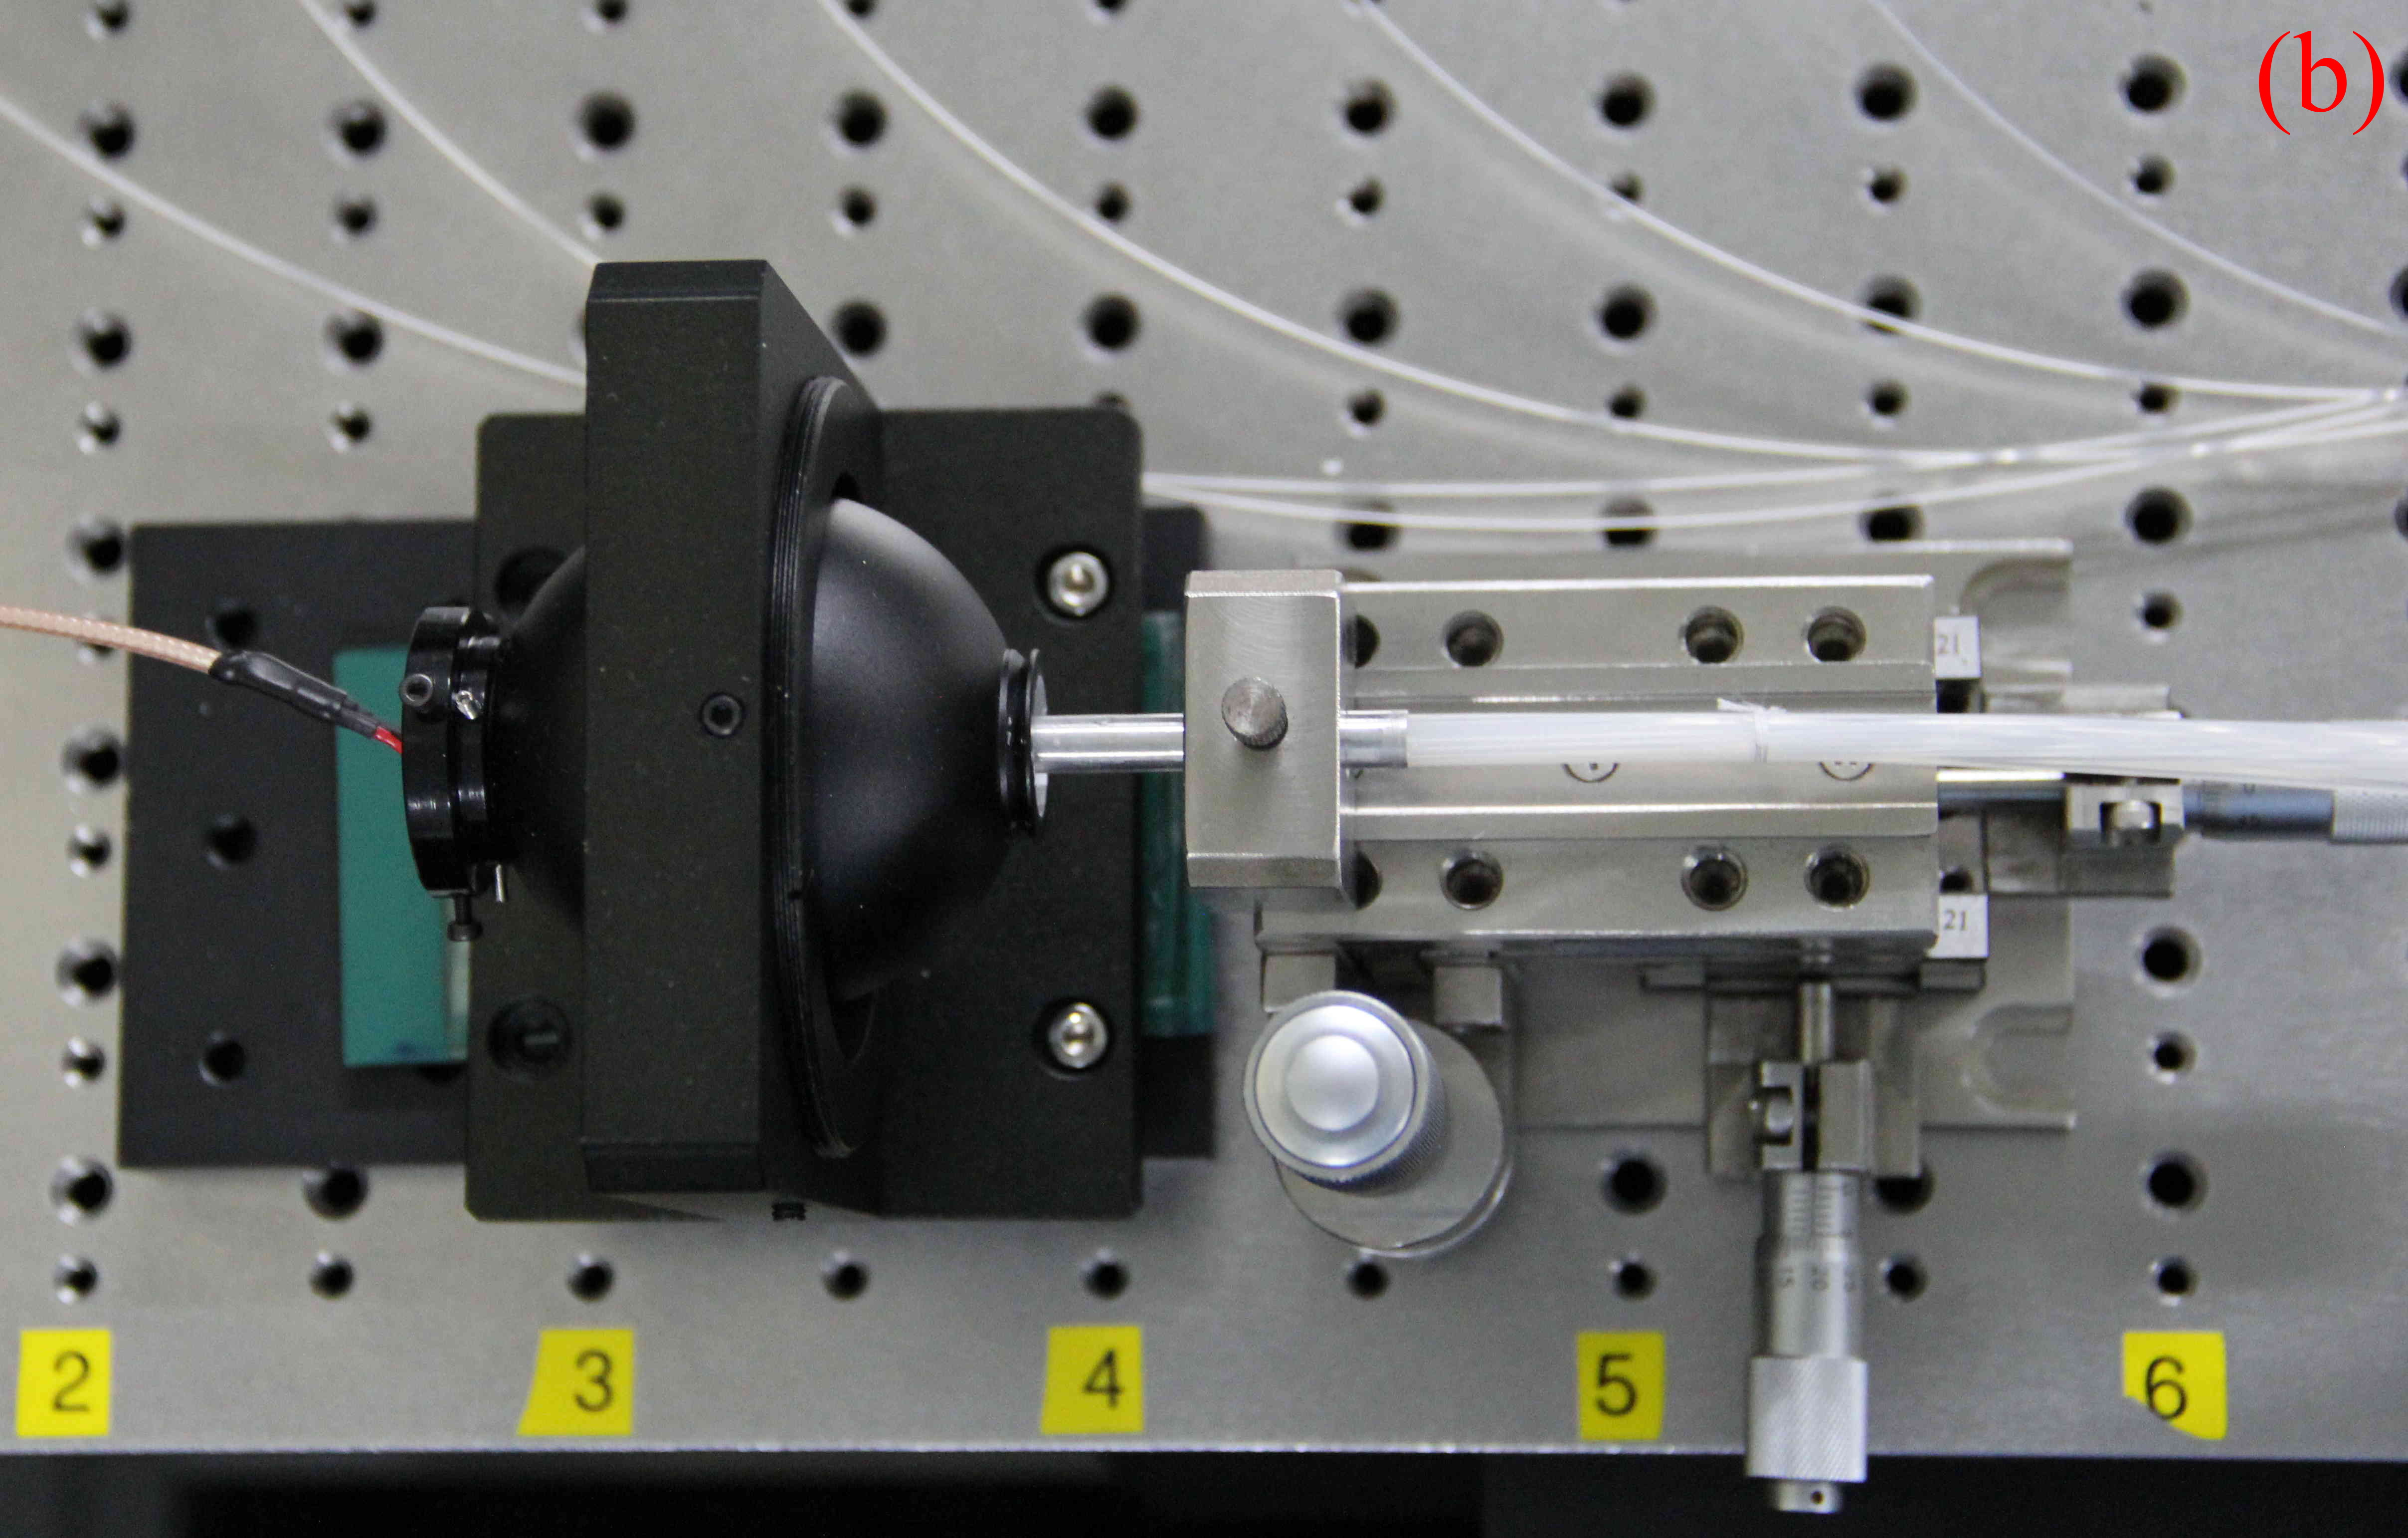
\includegraphics[width=80mm]{FIG3_b.jpg}
		\caption{Integration of the components.}
		\label{fig:FIG3_b}
	\end{subfigure}
	
	\caption{The light distribution system.}
	\label{fig:FIG3}
\end{figure}

The motorized and fixed stages form the main body of the test bench.
All other objects inside the light-tight container are mounted on the top of these two stages.
In particular, customized fixtures for the fibers, PMTs and the integration sphere have been designed for convenient and accurate positioning.
\begin{comment}
\begin{figure}[tbp]
\centering
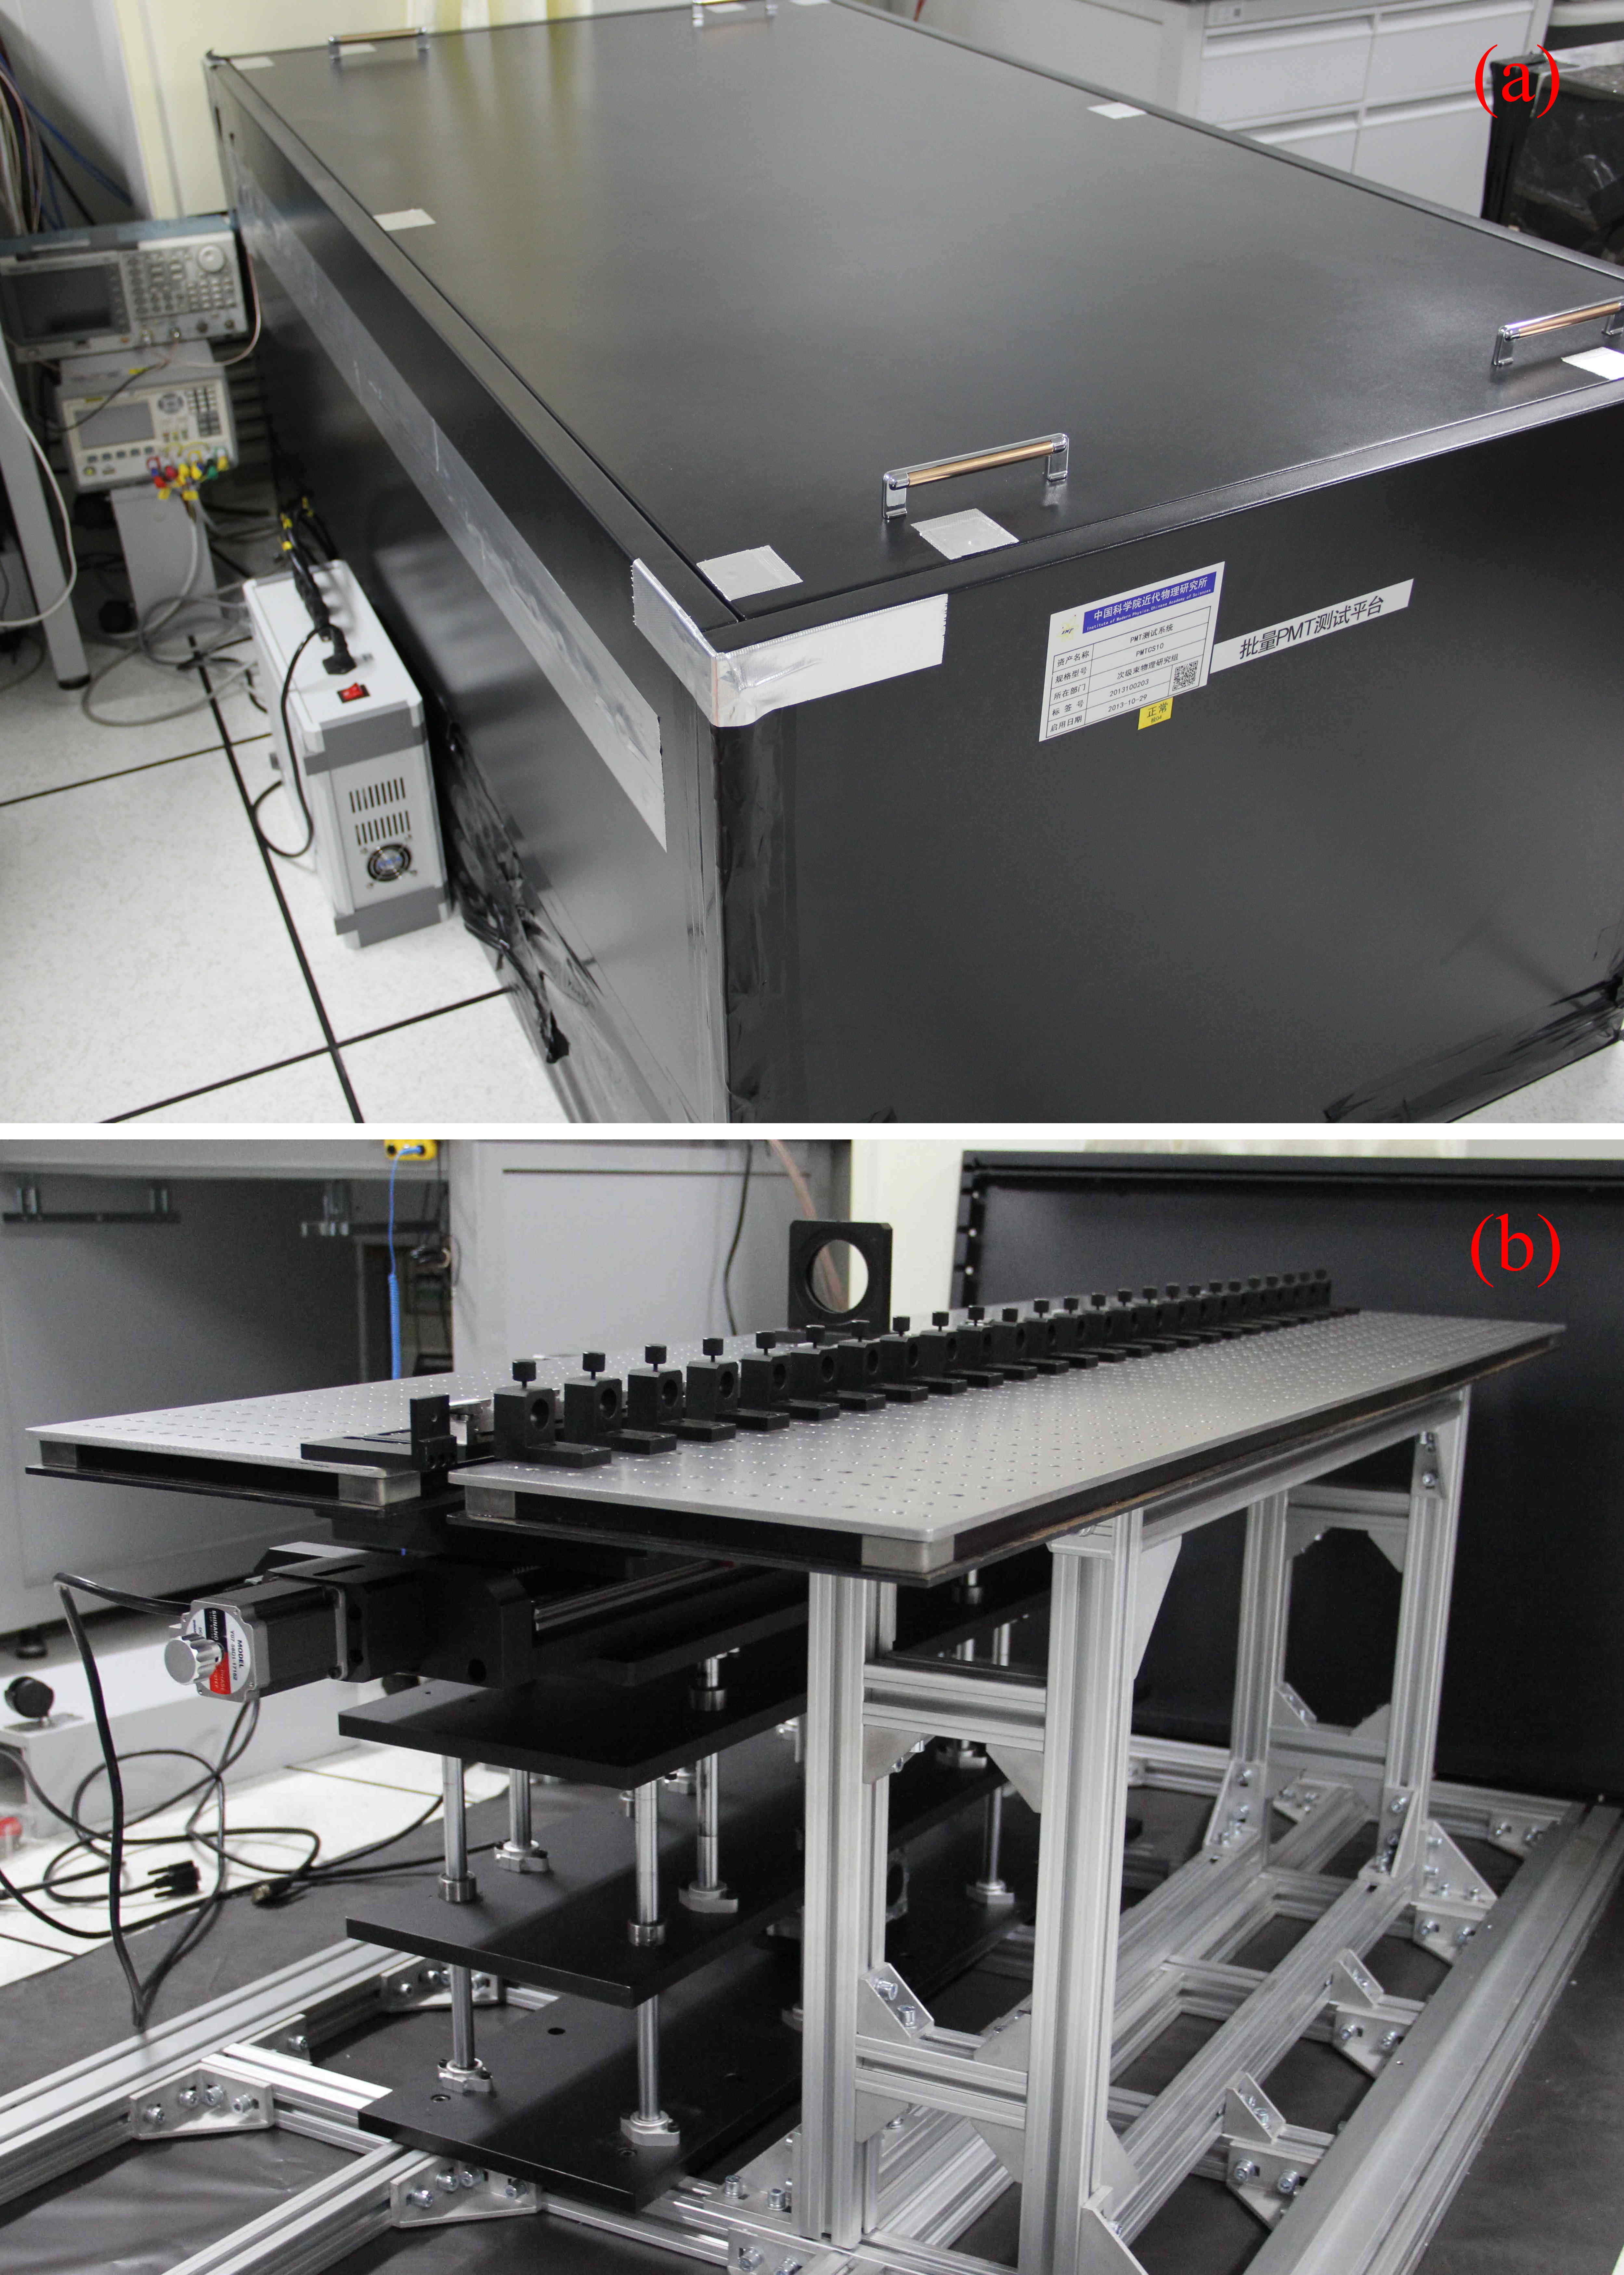
\includegraphics[width=90mm]{FIG2}
\caption{Motorized and fixed stages before assembly, with the fixtures for the integrating sphere, fibers and PMTs on the top.}
\label{fig:FIG2}
\end{figure} 
\end{comment}

As shown in Fig.~\ref{fig:FIG2_b}, both stages are covered with a $1560mm\times250mm$ optical breadboard. 
These breadboards are made of \SI{2.5}{cm} thick stainless steel, providing substantial resistance to deformation in this application. 
The grid pattern of tapped holes on their surface provide extra flexibility in the testing configuration as well as facilitates mounting/unmounting operations.

The load capacity of the motorized stage is \SI{30}{\kilo\gram} and it can perform a three-dimensional motion driven by three stepping motors. The minimum step size is \SI{1.56}{\micro\meter}.
The stage can move up to \SI{60}{\milli\meter} horizontally and \SI{70}{\milli\meter} vertically. This range is large enough to cover commonly used PMTs with diameters smaller than 2".
The stage can also move along the third direction for $15mm$, which is to control the gap between the fiber and the input window of PMT and to protect the fibers while mounting/unmounting the tubes.
All the stepping motors are controlled by a motion controller board MPC07SP from Leetro~\cite{leetro}, which possesses a PCI (Peripheral Component Interconnect bus) interface for remote control.

\subsection{Light source}
\label{sec:light_source}

A high-power blue LED (\SI{3}{\watt}, \SIrange{465}{485}{\nano\meter}) is adopted as the light source of the test bench.
The spectrum range of the LED is compatible with the spectral response of the most common photocathode.
It has been used before in the monitoring and calibration system of Neutron Wall Detector at IMP~\cite{yuyuhong_led} and proved to be suitable for massive light distribution.
The LED is fixed on a specially designed base using thermally conductive silicone rubber (see Fig.~\ref{fig:FIG3_a}), and then coupled to a \SI{5}{\centi\meter} diameter integrating sphere~\cite{integrating_sphere} directly.
The integrating sphere is a perfect light integrator and transforms the light output of LED into a uniform distribution.
Thus, the amount of photons reaching each fiber, which is a fixed fraction of the total output of the LED, is independent of position.
This makes the coupling between the light source and the fiber bundle much more easier and flexible, and stable light output difference between all the fiber channels can be achieved (see next section).

For PMT characterization, light pulses of short duration are needed.
%%%%%ADD 
The general purpose pulse generator, Tektronix AFG3252~\cite{afg3252}, is adopted to drive the LED directly.
Although it is not designed to be a dedicated LED driver, the performance of AFG3252 is quite satisfactory (an example is shown in Fig.~\ref{fig:FIG4}).
AFG3252 can adjust all the pulse parameters in a wide range with high precision. This is a critical feature for a test bench with an objective of versatility, as diverse requirements for the light pulses exist in different applications. 
Besides the LED driving pulse, AFG3252 can also output a synchronized pulse as the trigger signal to the DAQ, which will simplify the DAQ configuration in most cases. 

\begin{figure}[!htb]
	\centering
	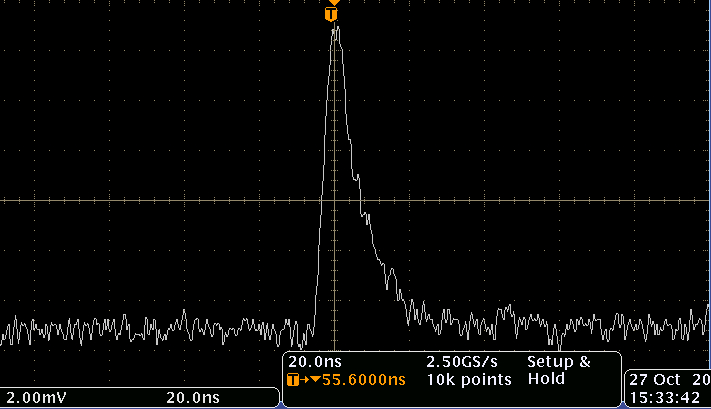
\includegraphics[width=85mm]{FIG4.jpg}
	%\captionsetup{justification=raggedright,singlelinecheck=false}
	\caption{An example of the PMT output waveform (extracted from dynode 8) in response to the light pulse drived by a square pulse of AFG3252 with \SI{30}{\nano\second} width and \SI{5}{\nano\second} leading/trailing time.}
	\label{fig:FIG4}
\end{figure} 

The uniformity of the light source has been verified by using the same optical fiber to scan the output port surface of the integrating sphere using a three-axes alignment stage. The other end of the fiber was then coupled to a fixed PMT to measure the light output intensity.
An uniformity within $\pm\SI{0.5}{\percent}$ has been reached, and this is sufficient to eliminate the spatial effect of light distribution.

\subsection{Fiber bundle}
\label{sec:fiber_bundle}

A bundle of 35 plastic clad silica fibers~\cite{optical_fibre} (25 for test channels, 2 for monitoring channels and 8 spares) is utilized to guide light pulses to each PMT.	Each fiber is \SI{1.5}{\meter} long and has a \SI{400}{\micro\meter} diameter core with a \SI{75}{\micro\meter} thick cladding, and the numerical aperture (NA) is 0.37.
The relatively large core and NA make the fiber an efficient light extractor of integrating sphere output. 

To protect the fibers from mechanical damage, both ends of the fiber bundle are coated with stainless steel ferrules (see Fig.~\ref{fig:FIG3_a}).
The bundle end is coupled to the center of the output port of the integrating sphere using a fiber alignment stage (see Fig.~\ref{fig:FIG3_b}).
On the other end, each fiber is fixed using a customized fiber holder which allows two-dimensional position adjustment, and is aligned to the center of the corresponding PMT input window with a precision of \SI{0.5}{\milli\meter}.

After coupling the fiber bundle to the integrating sphere, the light output difference between all the fiber channels was calibrated. 
The light output difference $\tau_{fiberid}$ is determined by comparing the light output intensity of each fiber channel ($L_{fiberid}$) to that of a reference channel ($L_{ref}$) under the same LED output as follows:
\begin{equation}
	\tau_{fiberid} = \frac{L_{fiberid}}{L_{ref}}
\end{equation} 
A fixed pulse generator setting was used to drive the LED, and the same PMT was used to record the output photons of each fiber successively.
The PMT (called testing PMT) was fixed and each fiber was aligned to the same photocathode position with a precision of \SI{0.1}{\milli\meter} using a fiber alignment stage.
Additionally, a separate PMT (called monitoring PMT) was used to monitor the light output fluctuation of the LED.
Thus ,the light output intensity of the fibers can be represented by the raw ADC counts of the testing PMT's signal after correcting the LED output fluctuation.
The result is shown in Fig.~\ref{fig:FIG5}, and a variance of \SI{10}{\percent} is observed among the fibers.
The same calibration procedure was performed at two LED output intensities, and the results are compatible with each other. 
Since the non-uniformity of the integrating sphere is negligible, the light output difference is a direct reflection of the transmission difference among the fibers themselves and shall be stable in a long period.
Thus, $\tau_{fiberid}$ is treated as a constant parameter and was used to normalize the light output intensity between different fiber channels in the measurement of the relative gain of PMT (see Section~\ref{sec:psd_gain})

\begin{figure}[!htb]
	\centering
	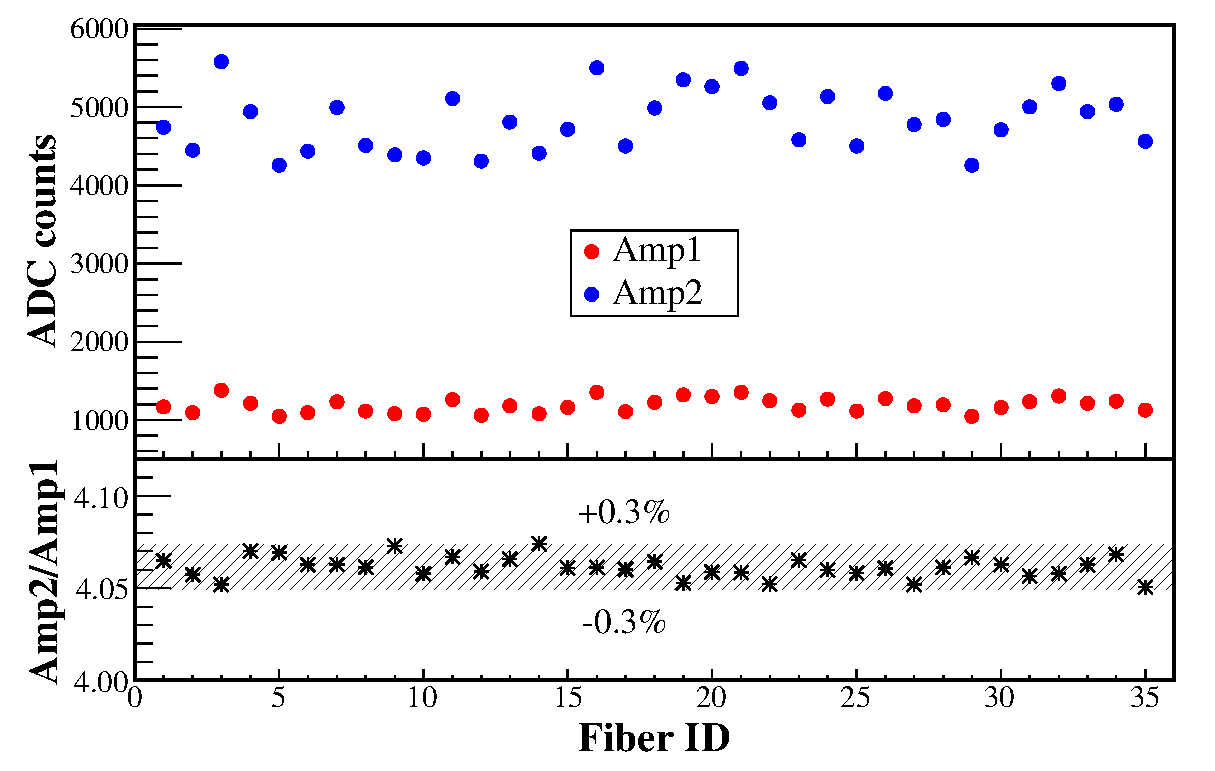
\includegraphics[width=85mm]{FIG5}
	%\captionsetup{justification=raggedright,singlelinecheck=false}
	\caption{Up: Light output of 35 fibers measured at two light intensities with an amplitude difference of about 4 times (the error bars are too small to be seen).
		Bottom: Ratio between the two measurements of each fiber, the results are consistent within $\pm\SI{0.3}{\percent}$.}
	\label{fig:FIG5}
\end{figure} 

\subsection{Software framework}
\label{sec:software}

The software for the test bench is developed under Windows using C++. It can be divided into three hierarchies as follows:
\begin{enumerate}
	\item \textit{Device abstraction}, which not only serves as an interface to the hardware, but also handles the abstraction of different types of devices. 
	\item \textit{Framework libraries}, which defines a general testing procedure and provides utility classes for configuration and management.
	\item \textit{User interface}, which provides command line based or graphical executable for user interaction. 
\end{enumerate}

Instead of developing a dedicated program each time a hardware changes, an abstraction of the devices is adopted to separate the testing procedure from hardware implementation details. 
Abstract classes are defined for the four types of essential equipments as shown in the rounded boxes in Fig.~\ref{fig:FIG1}.
New hardware of each type only needs to inherit from the corresponding abstract class and implement its interface methods and then registered in the singleton device management class \textit{PTDeviceManager} (\textit{PT} is the abbreviation for \textit{PMT Test}), leaving all other part of the software unchanged.
%Currently, concrete device classes for the hardware described in this section have all been implemented and fully tested.

\begin{figure*}[!htb]
	\centering
	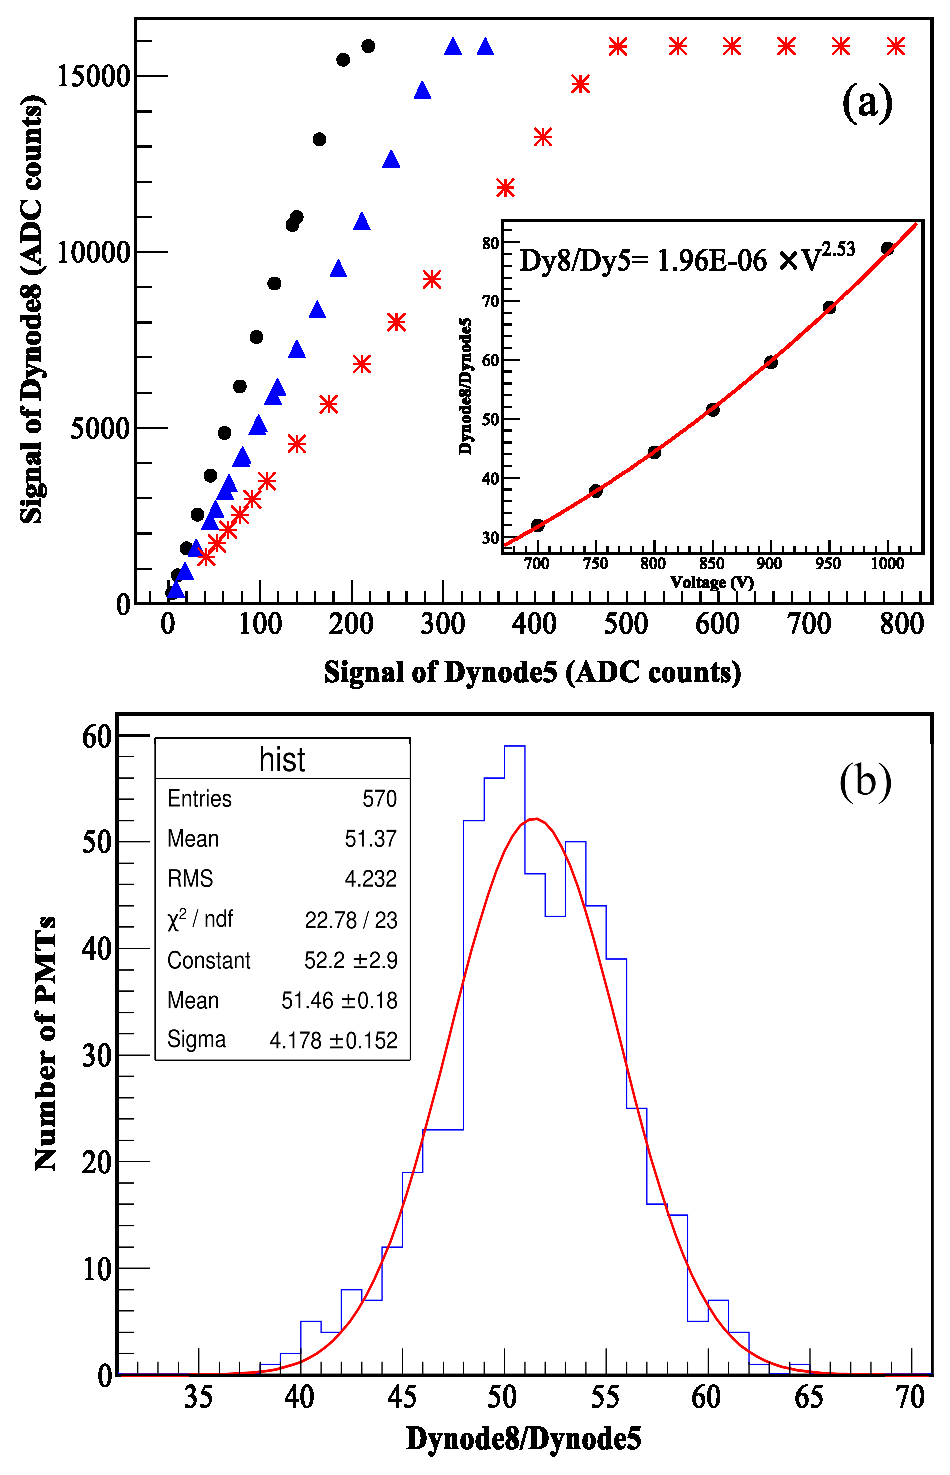
\includegraphics[width=120mm]{FIG6}
	\caption{General PMT testing framework. Fake code for a typical \textit{PTVTest} implementation is presented as an example.}
	\label{fig:FIG6}
\end{figure*}

Built upon the abstract device interface, a general testing framework is defined as shown in Fig.~\ref{fig:FIG6}.
\textit{PTVProgram} (\textit{V} in the class name indicates that it's an abstract class) represents the measurement for a specific characteristic of PMT, such as cathode uniformity, gain and so on.
\textit{PTVTest} is a subunit of \textit{PTVProgram}, which encapsulates the real device operations performed under a specific condition.
A \textit{PTVProgram} may consist of a series of \textit{PTVTest}s, which are invoked sequentially in a test loop.
For example, in cathode uniformity measurement, the stepping motor will move to a series of positions and the PMT response will be recorded by the DAQ at each position.
Here, device operations performed at each position constitute a \textit{PTVTest} and tests at all positions constitute a \textit{PTVProgram}.
Additional operations may be added in the \textit{PreTest} and \textit{PostTest} methods of \textit{PTVProgram}, which will be invoked before and after the test loop respectively.
\textit{PTVProgram}s of various testing objectives are finally chained together to constitute a complete characterization of PMT.

For easy usage, a light-weight user interface based on PDCurses~\cite{pdcurses} has also been developed.
This program features in device control, status monitoring and information logging.
%Thanks to the abstraction described above, the architecture of the program is rather independent of the specific hardware used and the testing programs performed.
A decoding function from binary file to ROOT file~\cite{root} is also incorporated into it for online monitoring.
However, more detailed analysis based on the ROOT file are considered project-specific, thus not included in the program. 

\section{Application in the construction of DAMPE-PSD}
\label{sec:application}

The PSD detector of the DAMPE project is a large-area plastic scintillator array. It aims for heavy ion charge measurement up to $Z=20$ as well as high energy e/$\gamma$ discrimination by measuring the deposited energy. PSD adopts the Hamamatsu R4443 PMT for the scintillation light detection, which is a ruggedized version of the previous R647~\cite{r4443}. The timing information from R4443 is not needed. To cover the large dynamic range, two dynodes, 5 and 8, are readout for each R4443 tube, 
and the signals are processed by a highly-sensitive ASIC chip (VA160~\cite{va160}, \SI{-3}{\pico\coulomb}$\sim$\SI{13}{\pico\coulomb}) followed by an ADC of 14~bits resolution~\cite{yanghaibo_fee}. 
Both the gain of dynode8 and the gain between dynode8 and dynode5 of each PMT need to be  measured during the characterization.

Concrete \textit{PTVProgram}s for gain, dynode8/dynode5 ratio and cathode uniformity measurements have been implemented.
To accommodate the low input range and obtain more realistic results, the ground-test electronics system of PSD~\cite{yanghaibo_fee} are utilized instead of the conventional CAMAC system. 
The ground-test system is mainly a copy of the real ones used in space, and a dedicated \textit{PTVDaq} class based on the NI-VISA library~\cite{ni_visa} has been implemented for it.
\begin{comment}
\begin{figure*}[!htb]
	\centering
	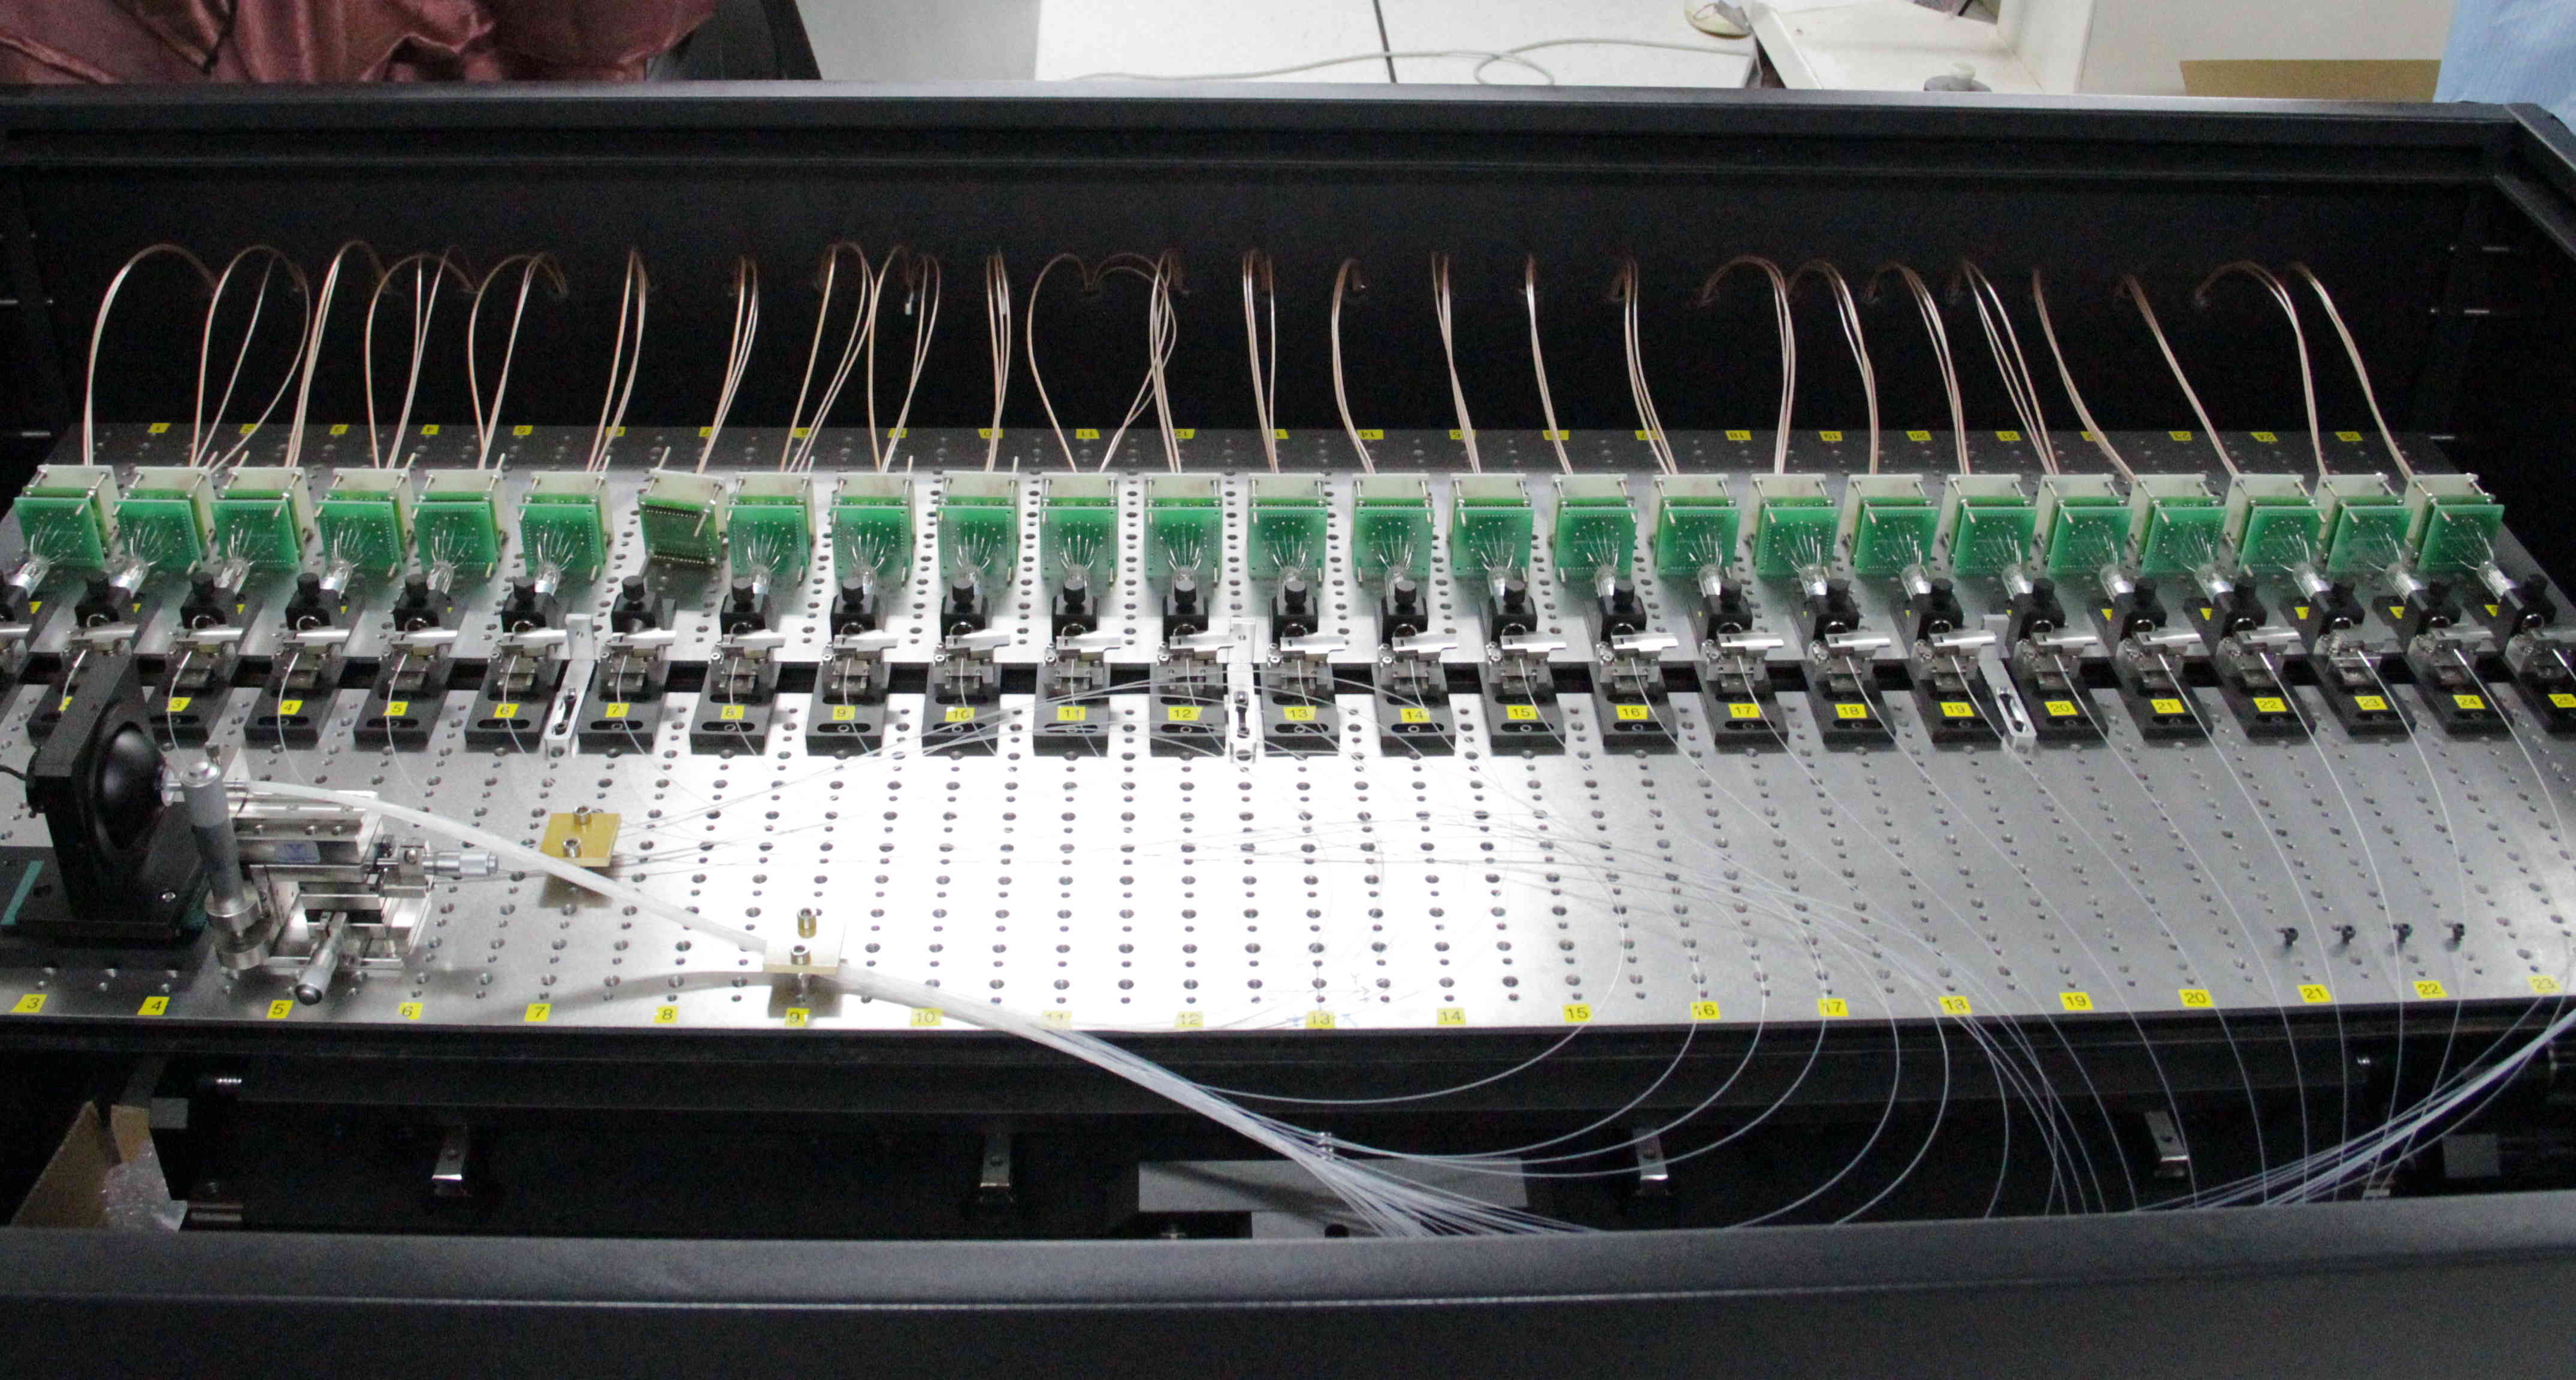
\includegraphics[width=0.8\textwidth]{integration1_crop.jpg}
	\caption{Testing of the R4443 tube}
	\label{fig:Integration}
\end{figure*}
\end{comment}

About 20 tubes are tested in a single run, and it takes normally five hours for a complete characterization, including two hour's warming time. 
28 test runs were performed in about a month, and totally 570 R4443 tubes have been characterized. 
All the data and analysis results have been stored in a MySQL database for easy query, and tubes for installation will be selected based on these data.

The selection procedure is not the subject of this article.
Here, only the major results are presented with a focus on the demonstration of the validity of the test bench. 

\subsection{Relative gain of dynode8}
\label{sec:psd_gain}

PSD requires a \SI{25}{\percent} uniformity in all detection units. 
Therefore, a relative measurement of the gain is adopted by comparing the responses of the PMTs to the same input light intensity.
A pusle generator setting with an intermediate light intensity is selected for this measurement, so that the responses of all the tested PMTs are within the linear range.


Due to the light output fluctuation of the LED between different test runs and the light output difference between different fiber channels, two corrections were applied to the measured raw data of each tested PMT to normalize the input light intensity and get the real response as follows: 
\begin{equation}
	A_{corr} = \frac{A_{raw}}{k_{runid}\tau_{fiberid}}
\end{equation} 
where $A_{raw}$ is the mean value of the raw ADC spectrum measured at the specified pulse generator setting,
$k_{runid}$ is the fluctuation of the LED output between different test runs,
$\tau_{fiberid}$ is the light output difference between fibers which has been measured in Section~\ref{sec:fiber_bundle}.
$k_{runid}$ is calculated at each test run using one of two monitoring PMTs on the fixed stage, it is the ratio between the response of the same monitoring PMT at the current run and that at the initial run.
The relative gain $G_{relative}$ can then be obtained by directly dividing the $A_{corr}$ of the tested PMT by that of a reference PMT.
%The reference PMT can be chosen arbitrarily and its working voltage will be determined by an cosmic ray test.

Seven different high voltages, from \SIrange{700}{1000}{\volt} with a \SI{50}{\volt} step, are scanned to obtain the gain variation as a function of supply voltage for each PMT, and the results are fitted using the power law function~\cite{hamamatsu}.
Based on the fitting result, the relative gain at any supply voltage can be calculated.
Distribution of the relative gain at 850V is shown in Fig.~\ref{fig:FIG7}, where the $A_{corr}$ of all tubes are divided by that of the tube with the smallest gain. 
A maximum of about 5.5 times difference in the gain has been observed.

\begin{figure}[!htb]
	\centering
	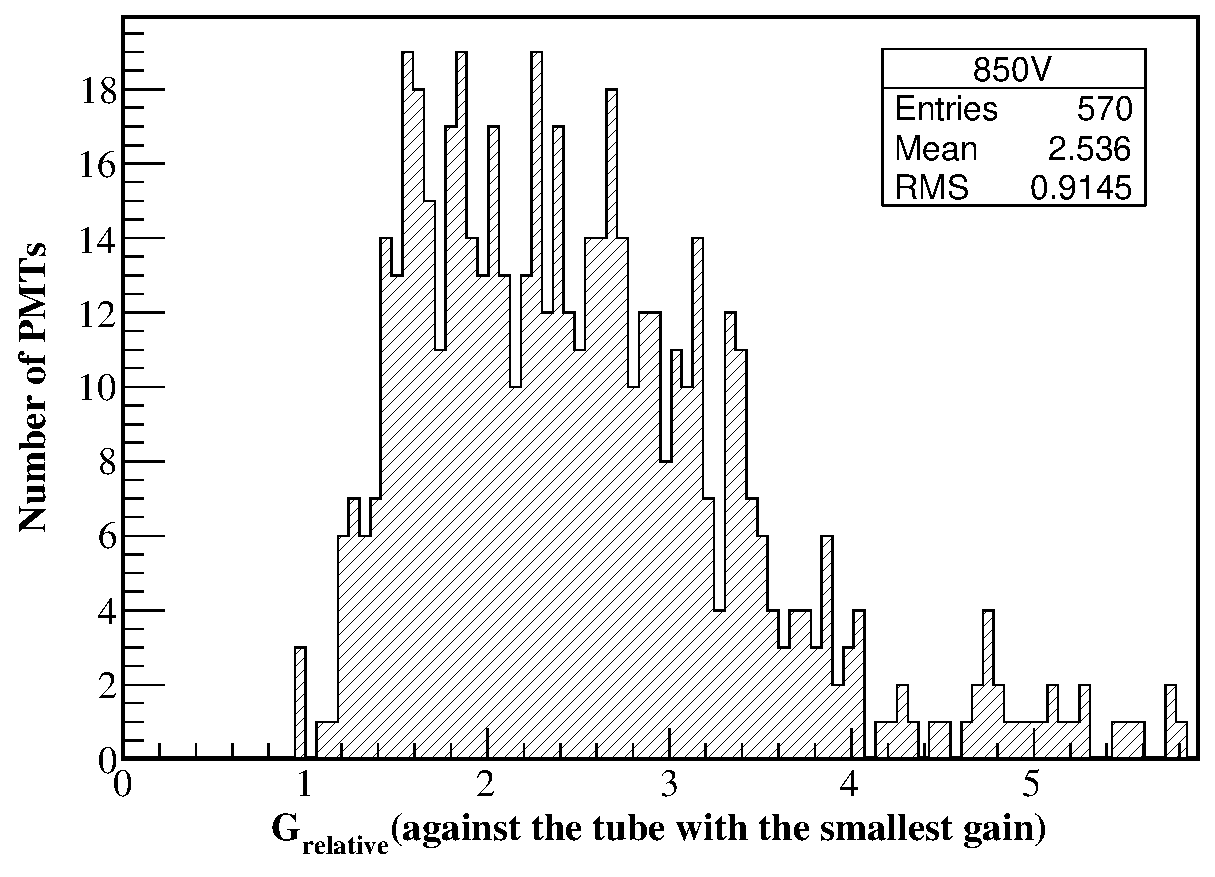
\includegraphics[width=85mm]{FIG7}
	%\captionsetup{justification=raggedright,singlelinecheck=false}
	\caption{Relative gain distribution measured at 850V (against the tube with the smallest gain).}
	\label{fig:FIG7}
\end{figure}

\subsection{Gain ratio between dynode8 and dynode5}
\label{sec:psd_dy58}

The gain ratio between dynode8 and dynode5 is measured by varying the light intensity in a large range until saturation of the dynode8 signal is observed.
The same procedure is repeated at 7 different supply voltages, from \SIrange{700}{1000}{\volt} with a \SI{50}{\volt} step, to obtain the dynode8/dynode5 dependency on voltage.
As with the gain of dynode8, the dependency can be fitted accurately with a power law function, as shown in the inset graph of Fig.~\ref{fig:FIG8_a}.
The ratio between the gain of dynode8 and dynode5 can then be calculated at any voltage value based on the fitting result.
As an example, the distribution of dynode8/dynode5 ratios at a certain supply voltage is shown in Fig.~\ref{fig:FIG8_b}.
%It can be seen that the variance is much smaller than that of gain.

\begin{comment}
\begin{figure}[tbp]
\centering
\includegraphics[width=\textwidth]{FIG6_h}
\caption{a) Example of the measurement of dynode8/dynode5 ratio.
Correlation between dynode5 and dynode8 at 1000V, 850V and 700V is presented, the saturation of dynode8 signal is clearly seen.
Power law fit to the measured dynode8/dynode5 of this tube at 7 voltage steps is shown in the inset graph. b) Distribution of the dynode8/dynode5 ratio at \SI{820}{\volt} calculated based on the fitted power law function.}
\label{fig:FIG6}
\end{figure} 
\end{comment}

\begin{figure}[!tb]
	
	\begin{subfigure}[t]{85mm}
		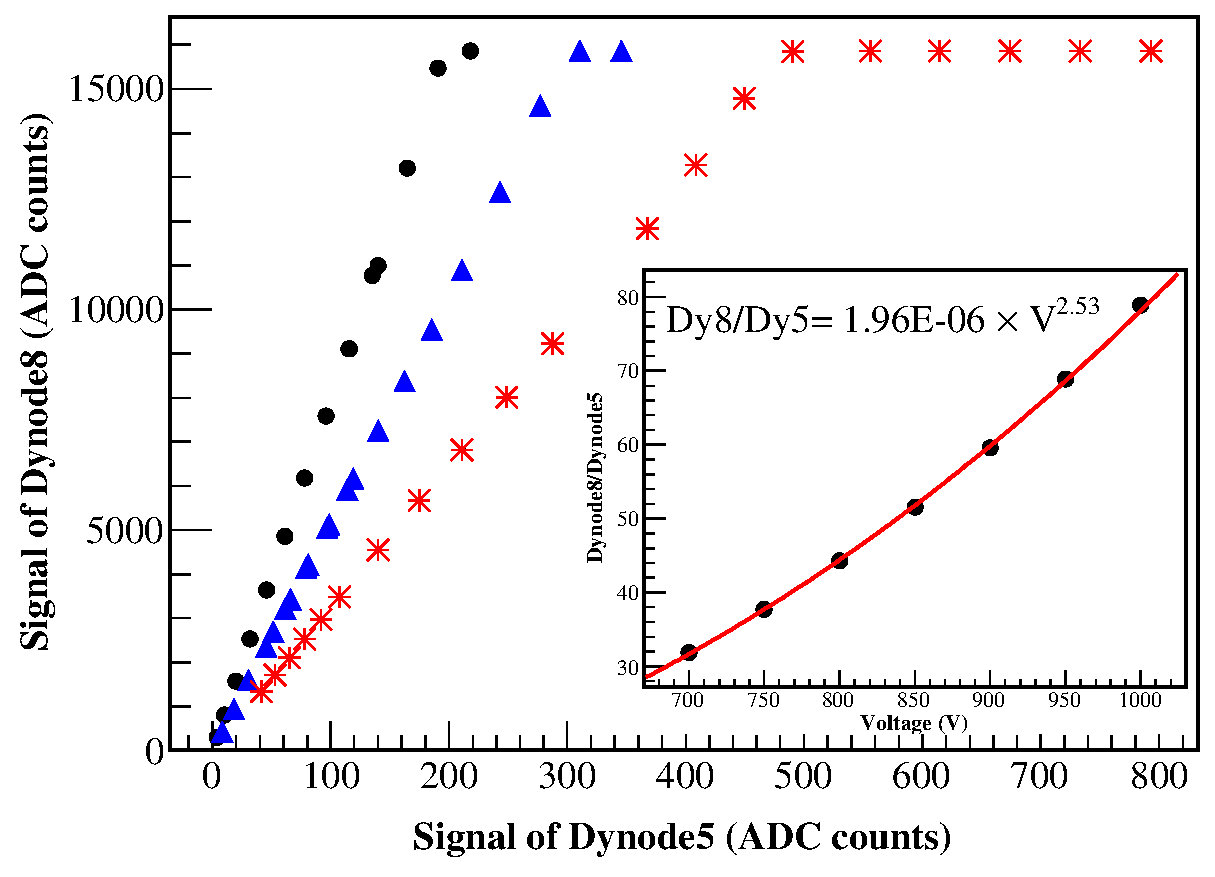
\includegraphics[width=85mm]{FIG8_a}
		%\captionsetup{justification=raggedright,singlelinecheck=false}
		\caption{An example of the measurement of dynode8/dynode5 ratio (the error bars are to small to be seen). Correlation between dynode5 and dynode8 at 1000V, 850V and 700V is presented, the saturation of dynode8 signal is clearly seen. Power law fit to the measured dynode8/dynode5 of this tube at 7 voltage steps is shown in the inset graph.}
		\label{fig:FIG8_a}
	\end{subfigure}
	\begin{subfigure}[t]{85mm}
		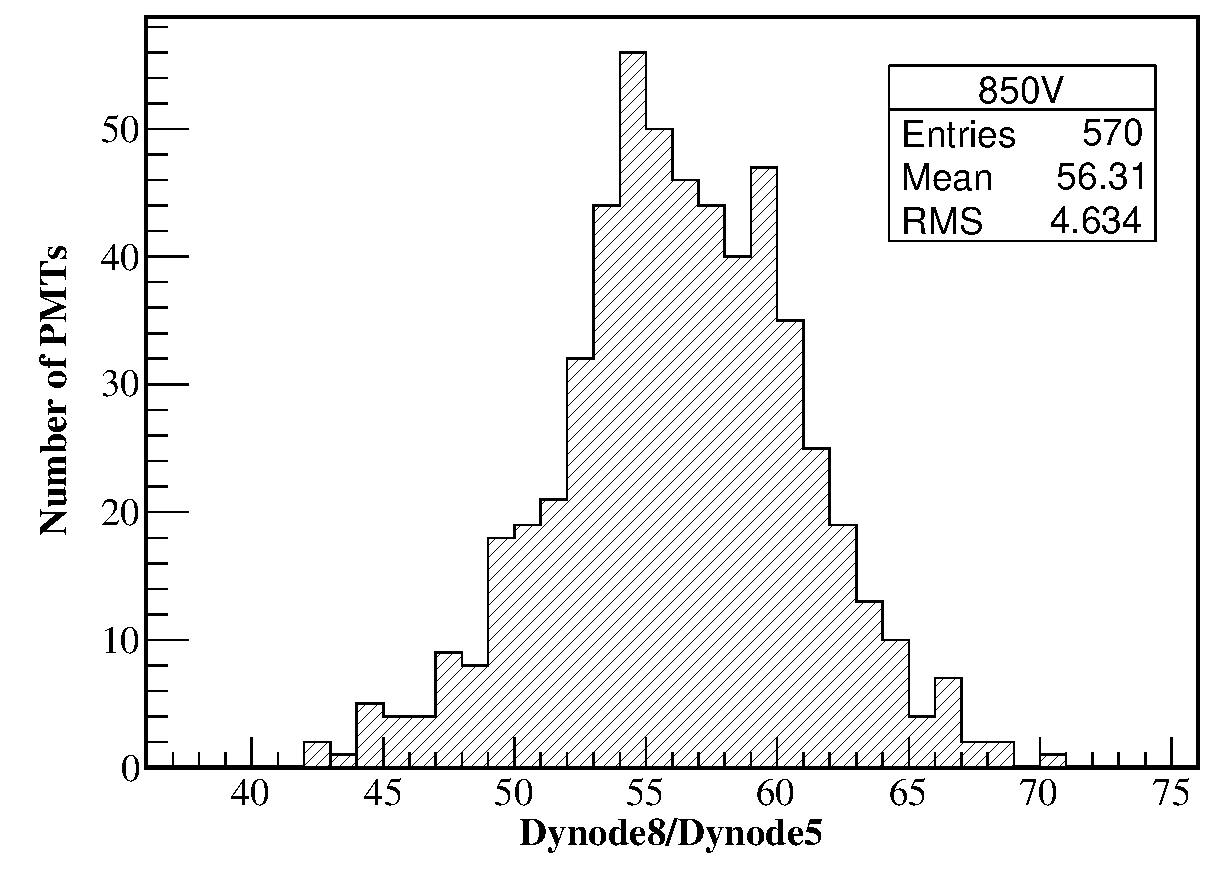
\includegraphics[width=85mm]{FIG8_b}
		\caption{Distribution of the dynode8/dynode5 ratio measured at \SI{850}{\volt}.}
		\label{fig:FIG8_b}
	\end{subfigure}
	
	\caption{Result of dynode8/dynode5 measurement.}
	%\caption{Left: An example of the measurement of dynode8/dynode5 ratio. Correlation between dynode5 and dynode8 at 1000V, 850V and 700V is presented, the saturation of dynode8 signal is clearly seen. Power law fit to the measured dynode8/dynode5 of this tube at 7 voltage steps is shown in the inset graph. Right: Distribution of the dynode8/dynode5 ratio measured at \SI{850}{\volt}.}
	\label{fig:FIG8}
\end{figure}

\subsection{Cathode uniformity}
\label{sec:psd_cathodescan}

\begin{figure}[!tb]
	\centering
	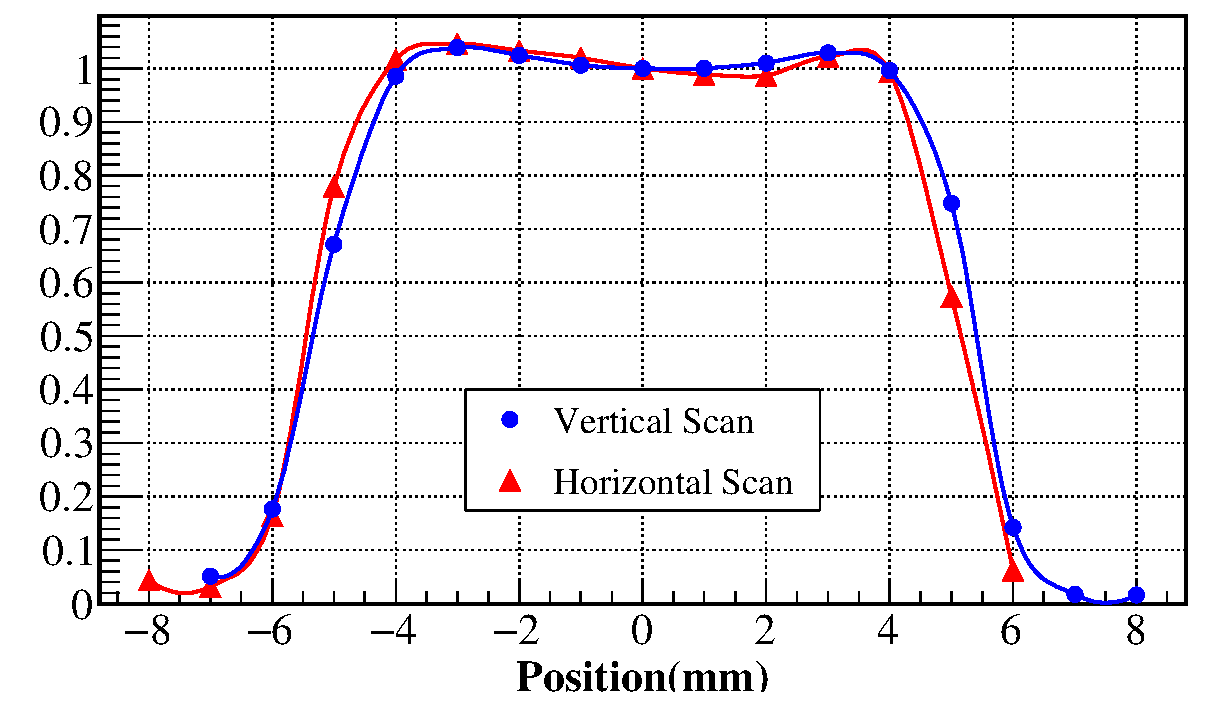
\includegraphics[width=85mm]{FIG9}
	%\captionsetup{justification=raggedright,singlelinecheck=false}
	\caption{A typical cathode uniformity of R4443.
		Relative gain at each position is normalized to the center of the input window.}
	\label{fig:FIG9}
\end{figure} 

The cathode uniformity of R4443 is also checked using the test bench, which has a minimum effective area of about \SI{10}{\milli\meter} in diameter.
The measurement is performed by scanning the input window of R4443 in two perpendicular directions with a step of \SI{1}{\milli\meter}.
At each position, the relative gain is measured at a fixed light source setting according to the method described in Section~\ref{sec:psd_gain}, and a typical result is shown in Fig.~\ref{fig:FIG9}.

The relative gain at each position is proportional to the total efficiency of light transmission, photoelectric conversion and electron collection at this point.
A rapid drop of this efficiency is observed at the edge of the cathode surface. 
Defining the uniform region as a region with the efficiency fluctuation less than \SI{10}{\percent}, it is found that only \SI{75}{\percent} of the tested PMTs can have a uniform region larger than \SI{9}{\milli\meter} in diameter. 

\subsection{Stability of the test bench}
\label{sec:stability}

The stability of the test bench during the PMT characterization for DAMPE-PSD can be extracted using the two fixed monitoring PMTs.

\begin{figure}[!htb]
	\centering
	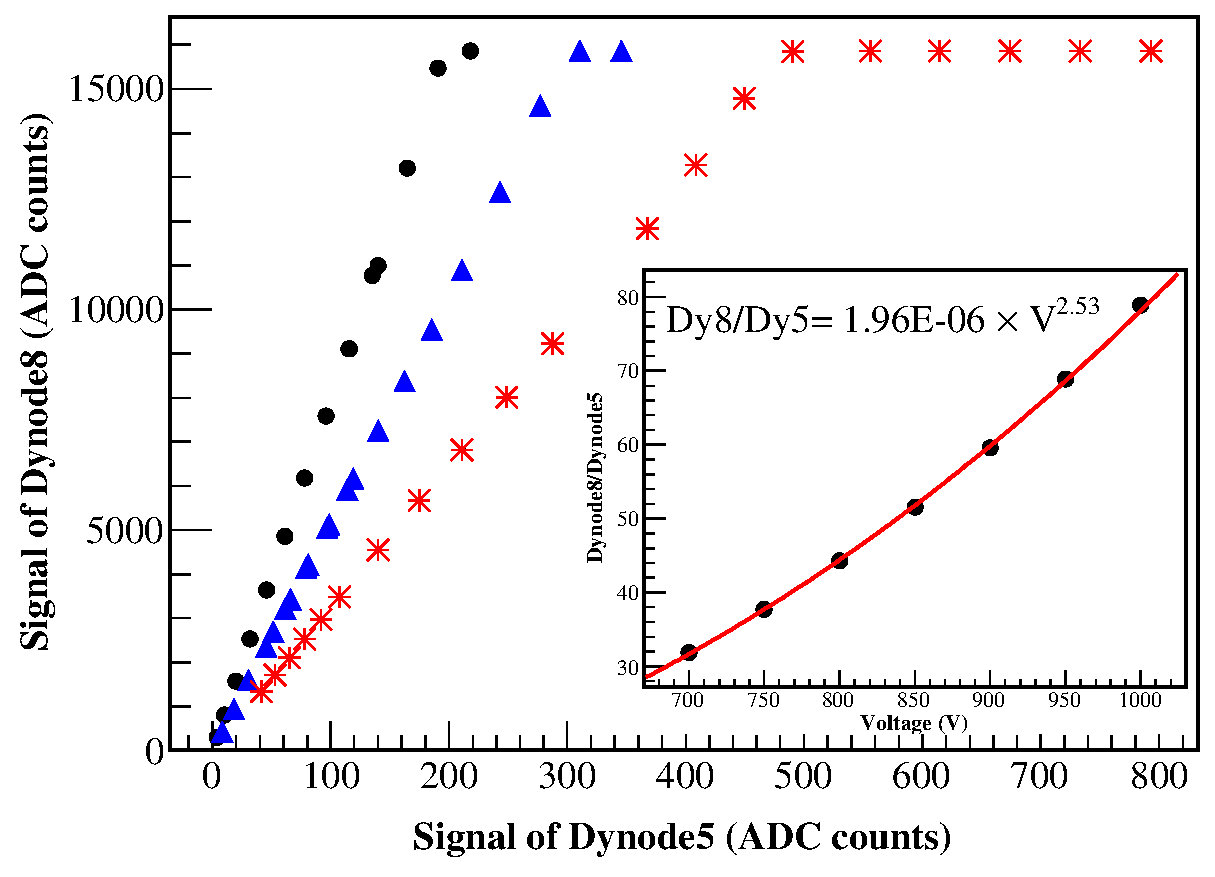
\includegraphics[width=85mm]{FIG10}
	%\captionsetup{justification=raggedright,singlelinecheck=false}
	\caption{Stability of the LED monitored by reference PMT2 at 900V (other voltage values give the same results) . Red line : $A_{raw}$ before light intensity correction. Blue line : $A_{corr}$ using reference PMT1 for light intensity correction. All the data points are all normalized to the first test run.}
	\label{fig:FIG10}
\end{figure} 

By checking the response of the monitoring PMTs with the same pulse generator setting at different test runs, a maximum variation of \SI{4}{\percent} in the output light intensity of the LED is observed during a period of about one month.
Light output fluctuation of the LED can be corrected using the method described in Section~\ref{sec:psd_gain} where $\tau_{fibreid}$ correction is not needed because the same fiber channel is utilized.
As two reference PMTs exists, this method can be validated by using one of them for output light correction and then checking the relative gain of the other. 
After the correction, the stability of the LED can be controlled within $\pm\SI{0.5}{\percent}$ as shown in Fig.~\ref{fig:FIG10}.

Monitoring PMTs underwent the same testing procedures as the tubes under test.
Measurement results of the parameters of the monitoring PMTs in different test runs can be filled together, and the spread of the distribution is an indication of the uncertainty of the testing method.
In this way, the uncertainty of the dynode8/dynode5 measurement is found to be \SI{1.59}{\percent}, and the uncertainty of relative gain measurement is \SI{0.53}{\percent}. 
	
\section{Summary}
\label{sec:summary}
A PMT test bench system based on the modular design pattern has been developed at IMP, CAS.
It can characterize 25 PMTs simultaneously and features in two-dimensional photocathode position scanning, configurable light pulse setting and highly automatic software control. A total of 570 R4443 PMT for the DAMPE-PSD detector have been characterized successfully using the test bench and the stability of the test bench was proven to be within $\pm\SI{0.5}{\percent}$.
Considering the flexible and open platform it possesses, the test bench shall be useful for any other experiments that need massive PMT characterization. 

\begin{comment}
\acknowledgments
This work was supported by the Strategic Priority Research Program of the Chinese Academy of Science under Grant No. XDA04040202-3.
\end{comment}

\begin{comment}
\begin{thebibliography}{99}
\bibitem{bib:1} Baran V, Cabibbo M, Colonna M, \emph{et al}. The dynamical dipole mode in dissipative heavy-ion collisions.  Nucl Phys A, 2001, {\bf 679}: 373--392. \href{http://dx.doi.org/10.1016/S0375-9474(00)00365-1}{DOI: 10.1016/S0375-9474(00)00365-1}
\bibitem{bib:2} Tao C, Ma Y G, Zhang G Q, \emph{et al}. Pygmy and giant dipole resonances by Coulomb excitation using a quantummolecular dynamics model. Phys Rev C, 2013, {\bf 87}: 014621. \href{http://dx.doi.org/10.1103/PhysRevC.87.014621}{DOI: 10.1103/PhysRevC.87.014621}
\bibitem{bib:3} Samson J A, Ederer D L. Vacuum ultraviolet spectroscopy I. New York (USA): Academic Press, 1998, 379--388.
\bibitem{bib:4} Mettam G R, Adams L B. How to prepare an electronic version of your article. In: Jones B S, Smith R Z, editors. Introduction to the electronic age. New York (USA): E-Publishing Inc, 1999, 281--304.
\bibitem{bib:5} Zhang B, Harada T, Hirahara D. N6P1042: Experimental Study of Self-Leveling Behavior in Debris Bed, the Sixth Japan-Korea Symposium on Nuclear Thermal Hydraulics and Safety (NTHAS6), Okinawa, Japan, Nov.~24--27, 2008.
\end{thebibliography}
\end{comment}

\begin{thebibliography}{99}
	\bibitem{barnhill_testing_2008} Barnhill D, Suarez F, Arisaka K, \emph{et al}. Testing of photomultiplier tubes for use in the surface detector of the {Pierre} {Auger} observatory. Nucl. Instrum. Meth. A, 2008, {\bf 591}: 453--466.
	\href{http://dx.doi.org/10.1016/j.nima.2008.01.088}{DOI: 10.1016/j.nima.2008.01.088}
	\bibitem{akgun_complete_2005} Akgun U, Ayan A S, Bruecken P, \emph{et al}. Complete tests of 2000 {Hamamatsu} {R}7525HA phototubes for the {CMS}-{HF} {Forward} {Calorimeter}. Nucl. Instrum. Meth. A, 2005, {\bf 550}: 145--156.
	\href{http://dx.doi.org/10.1016/j.nima.2005.03.171}{DOI: 10.1016/j.nima.2005.03.171}
	\bibitem{adragna_pmt-block_2006} Adragna P, Antonaki A, Boudagov I, \emph{et al}. A {PMT}-{Block} test bench. Nucl. Instrum. Meth. A, 2006, {\bf 564}: 597--607.
	\href{http://dx.doi.org/10.1016/j.nima.2006.03.045}{DOI: 10.1016/j.nima.2006.03.045}
	\bibitem{Chang_Jin_dampe} Chang J, Dark matter particle explorer: the first chinese cosmic ray and hard $\gamma$-ray detector in space. Chinese Journal of Space Science, 2014, {\bf 34}: 550-556.
	\href{http://dx.doi.org/10.11728/cjss2014.05.550}{DOI: 10.11728/cjss2014.05.550}
	\bibitem{yuyuhong_led} Yu Y H, Xu H G, Zhan W L, \emph{et al}. Study of the LED based light calibration system for neutron wall detector. High Energ Phys. Nuc., 2007, {\bf 31}: 581-585.
	\bibitem{sy1527lc} {CAEN S.p.A.}, Low cost universal multichannel power supply system. \href{http://www.caen.it/csite/CaenProd.jsp?idmod=491&parent=20}{http://www.caen.it}
	\bibitem{cc_usb} {W-IE-NE-R Plein \& Baus GmbH.}, {CC-USB CAMAC controller with USB interface}. \href{http://www.wiener-d.com/sc/modules/camac--modules/cc-usb.html}{http://www.wiener-d.com}
	\bibitem{leetro} {Leetro Automation Co. Ltd.}, {MPC07SP motion control board}. \href{http://www.leetro.com/english/}{http://www.leetro.com}
	\bibitem{integrating_sphere} {Mulansphere Co. Ltd.}, {Customized \SI{5}{cm} aluminum-alloy integrating sphere}. \href{http://mulansphere.com/e-index.html/}{http://mulansphere.com}
	\bibitem{afg3252} {Tektronix Company}, {AFG3000 series arbitrary/function generators quick start user manual}. \href{http://www.tek.com/signal-generator/afg3000-function-generator/}{http://www.tek.com}
	\bibitem{optical_fibre} Nanjing Chunhui Science and Technology Industrial Co. Ltd., Customized plastic-clad silica fiber-bundle.  \href{http://www.china-light-guides.com/}{http://www.china-light-guides.com}
	\bibitem{pdcurses} PDCurses,  Public domain curses library for DOS, OS/2, Win32, X11 and SDL. \href{http://pdcurses.sourceforge.net/}{http://pdcurses.sourceforge.net}
	\bibitem{root} CERN,  ROOT data analysis framework. \href{https://root.cern.ch/}{https://root.cern.ch}
	\bibitem{r4443} Hamamatsu Photonics K. K., R647 data sheet.
	\href{http://www.hamamatsu.com/us/en/R647.html}{http://www.hamamatsu.com/us/en/R647.html}
	\bibitem{va160} Integrated Detector Electronics AS., A 32-channel ASIC chip for PMT spectrometer readout with trigger. \href{http://www.ideas.no/products/ide3160-2/}{http://www.ideas.no}
	\bibitem{yanghaibo_fee} Yang H B, Signals reading method and circuit design for multiple detection unit based on the advanced {ASIC} chips, Ph.D. Thesis, The University of Chinese Academy of Sciences, 2014.
	\bibitem{ni_visa} National Instruments Co.,  National Instruments {VISA} library. \href{http://www.ni.com/visa/}{http://www.ni.com/visa}
	\bibitem{hamamatsu} Hamamatsu Photonics K. K., Photomultiplier tubes: basics and applications, 3rd edition.
	\href{http://www.hamamatsu.com/resources/pdf/etd/PMT_handbook_v3aE.pdf}{http://www.hamamatsu.com/resources}
\end{thebibliography}


%\bibliography{mybib}

\end{document}
